\chapter{Introduction and Background}\label{chap:intro}

\section{Clinical Context and Problem Definition}

Meniscal injuries are among the most frequently encountered knee pathologies in orthopedic practice, often resulting in chronic pain, joint dysfunction, and long-term degenerative changes~\cite{mordecai2014treatmentmeniscal, beeler2020meniscussizing, baek2015meniscustissue, abdelgaied2015comparisonbiomechanical}.
The unique challenges in meniscus healing stem from its limited vascular supply, particularly in the inner regions where most injuries occur~\cite{athanasiou2009engineeringknee, makris2011kneemeniscus, tran2020comprehensivereview}.
This avascularity, combined with the constant mechanical loads experienced during daily activities, creates a complex healing environment that often leads to poor outcomes~\cite{makris2011kneemeniscus, athanasiou2009engineeringknee, bahcecioglu20193dprinted}.
Given the high prevalence of meniscus injury combined with these biological and mechanical challenges that limit the success of current surgical techniques, a viable alternative is in high demand~\cite{mordecai2014treatmentmeniscal, a.murphy20243dprintedvariable, baek2015meniscustissue}.



As illustrated in Figure~\ref{fig:ch1_clinicalimpact}, meniscal injuries impose a substantial burden across clinical, demographic, economic, and long-term health dimensions~\cite{mordecai2014treatmentmeniscal, beeler2020meniscussizing, baek2015meniscustissue, abdelgaied2015comparisonbiomechanical}.
Clinically, meniscal injuries are the most common sports-related injury and necessitate more than 750,000 surgical interventions annually in the United States alone, with partial meniscectomy remaining the most common procedure despite its association with significant long-term complications~\cite{mordecai2014treatmentmeniscal, beeler2020meniscussizing, baek2015meniscustissue}.
The demographic impact is broad, affecting a wide range of age groups from young athletes to elderly patients, each presenting different activity profiles that necessitate tailored treatment strategies~\cite{mordecai2014treatmentmeniscal, baek2015meniscustissue, abdelgaied2015comparisonbiomechanical}.
Economically, meniscal injuries contribute to substantial healthcare costs, including direct surgical expenses, rehabilitation services, and lost productivity, with overall expenditures estimated to reach several billion dollars annually~\cite{beeler2020meniscussizing, mordecai2014treatmentmeniscal, baek2015meniscustissue}.
Moreover, the long-term consequences are profound, as meniscectomy significantly increases the risk of post-traumatic osteoarthritis, ultimately leading to a decreased quality of life and, in many cases, the eventual need for total knee replacement~\cite{mordecai2014treatmentmeniscal, abdelgaied2015comparisonbiomechanical, baek2015meniscustissue}.

\begin{figure}[H]
    \centering
    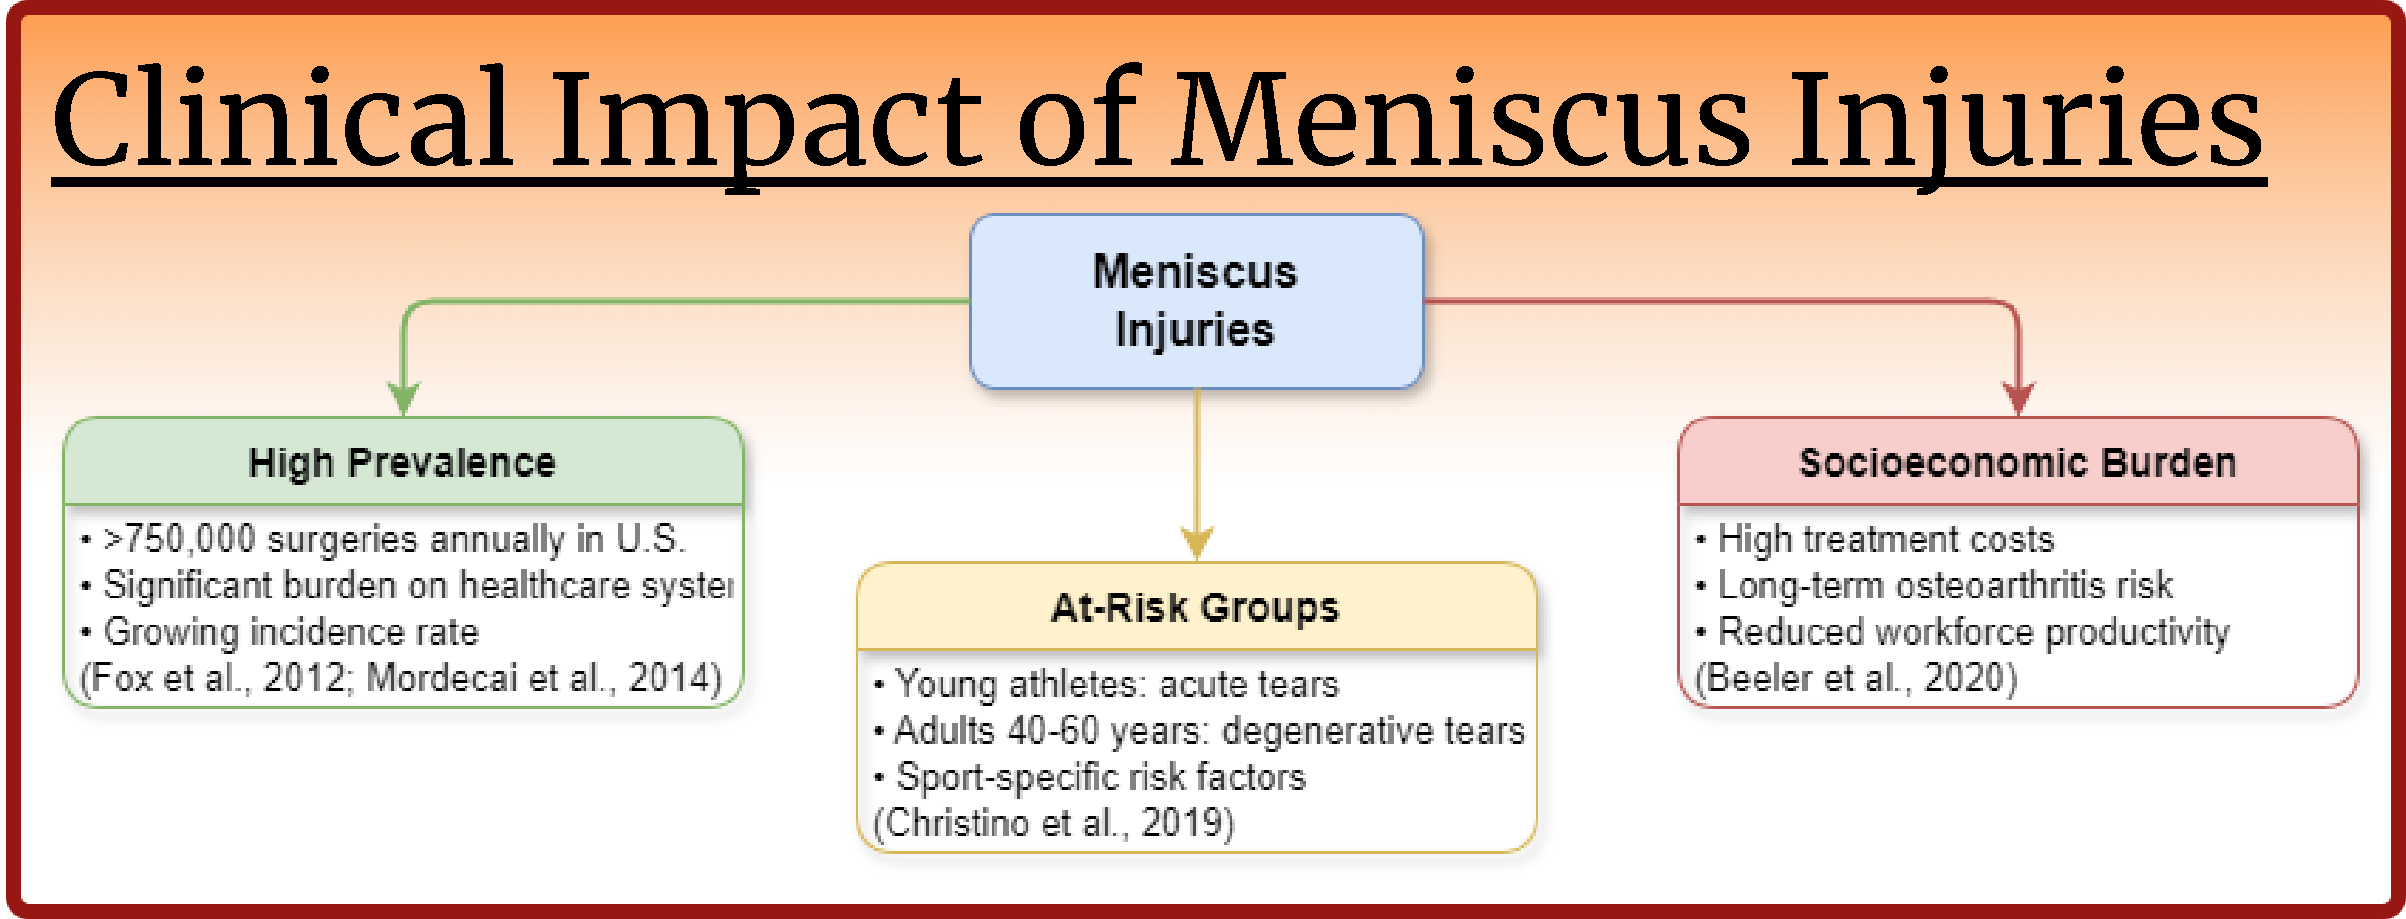
\includegraphics[width=1\linewidth]{figures/intro/ch1_clinicalimpact.pdf}
    \caption[Clinical Impact of Meniscal Injuries]{\textbf{Clinical Impact of Meniscal Injuries.} Clinical impact of meniscus injuries, highlighting their high prevalence, identification of at-risk groups, and associated socioeconomic burden. Meniscal injuries contribute significantly to healthcare demands and long-term disability, particularly due to their association with osteoarthritis and loss of productivity. (Adapted from Mordecai et al., Beeler et al., and Abdelgaied et al.)}
    \label{fig:ch1_clinicalimpact}
\end{figure}

Together, these burdens underscore the urgent need for regenerative solutions that not only restore mechanical function but also mitigate the long-term risks of joint degeneration~\cite{a.murphy20243dprintedvariable, bahcecioglu20193dprinted, baek2015meniscustissue}.
\newpage
\subsection{Types of Meniscal Injuries and Clinical Challenges}
Meniscal tears are the most common form of meniscal injury and can arise from both traumatic events and chronic degenerative changes~\cite{mordecai2014treatmentmeniscal, baek2015meniscustissue, abdelgaied2015comparisonbiomechanical}.
Several distinct tear patterns are recognized, as illustrated in Figure~\ref{fig:ch1_injuriesandmechanics}, each affecting knee function differently and influencing treatment strategies~\cite{makris2011kneemeniscus, szojka2017biomimetic3d, athanasiou2009engineeringknee}:

\begin{itemize}
    \item \textbf{Radial Tears:} Extend from the inner margin outward, disrupting the circumferential fibers essential for hoop stress generation~\cite{szojka2017biomimetic3d, makris2011kneemeniscus}.
    \item \textbf{Longitudinal Tears:} Run parallel to the meniscal curvature, often occurring in the more vascularized peripheral regions where healing potential is greater~\cite{makris2011kneemeniscus, athanasiou2009engineeringknee}.
    \item \textbf{Oblique (Flap) Tears:} Create unstable segments that may impinge during movement, causing mechanical symptoms~\cite{mordecai2014treatmentmeniscal, baek2015meniscustissue}.
    \item \textbf{Horizontal Tears:} Commonly associated with degenerative changes~\cite{makris2011kneemeniscus, athanasiou2009engineeringknee}.
    \item \textbf{Complex Tears:} Involve combinations of radial, longitudinal, and horizontal components~\cite{makris2011kneemeniscus, baek2015meniscustissue}.
    \item \textbf{Bucket Handle Tears:} Result in mechanical locking and severe mechanical dysfunction~\cite{mordecai2014treatmentmeniscal, baek2015meniscustissue}.
\end{itemize}

Understanding the morphology and location of meniscal injuries is essential, as healing potential varies markedly between the vascularized (red zone) and avascular (white zone) regions~\cite{athanasiou2009engineeringknee, tran2020comprehensivereview, makris2011kneemeniscus, baek2015meniscustissue}.
Accurate diagnosis and classification are therefore critical for selecting appropriate treatment approaches and optimizing clinical outcomes~\cite{mordecai2014treatmentmeniscal, abdelgaied2015comparisonbiomechanical}.

\subsection{Current Treatment Limitations and Unmet Needs}

The clinical challenges associated with meniscal injuries extend beyond the initial injury to encompass the limitations of current treatment approaches~\cite{mordecai2014treatmentmeniscal, kwon2019surgicaltissue, baek2015meniscustissue}. While surgical interventions can provide symptomatic relief, they often fail to address the underlying biomechanical dysfunction and may accelerate joint degeneration~\cite{athanasiou2009engineeringknee, abdelgaied2015comparisonbiomechanical, mordecai2014treatmentmeniscal}. The lack of effective regenerative solutions creates a significant unmet clinical need that impacts millions of patients worldwide~\cite{beeler2020meniscussizing, baek2015meniscustissue}.

Current treatment strategies face several fundamental limitations:

\begin{itemize}
    \item \textbf{Incomplete Functional Restoration:} Most treatments fail to fully restore the complex biomechanical functions of the native meniscus~\cite{makris2011kneemeniscus, athanasiou2009engineeringknee, abdelgaied2015comparisonbiomechanical}
    \item \textbf{Accelerated Joint Degeneration:} Meniscectomy and inadequate repairs often lead to early osteoarthritis~\cite{mordecai2014treatmentmeniscal, abdelgaied2015comparisonbiomechanical, baek2015meniscustissue}
    \item \textbf{Limited Regenerative Capacity:} Current approaches do not promote true tissue regeneration~\cite{kwon2019surgicaltissue, li2024advancedhydrogel, baek2015meniscustissue}
    \item \textbf{Patient-Specific Challenges:} Treatment success varies significantly based on patient age, activity level, and injury characteristics~\cite{mordecai2014treatmentmeniscal, beeler2020meniscussizing, tran2020comprehensivereview}
    \item \textbf{Long-term Durability Issues:} Many interventions provide temporary relief but fail to prevent long-term complications~\cite{ghodbane2019partialmeniscus, sun2017overviewscaffold, kwon2019surgicaltissue}
\end{itemize}

These limitations highlight the critical need for next-generation tissue engineering approaches that can address both the mechanical and biological requirements for successful meniscal replacement~\cite{a.murphy20243dprintedvariable, bahcecioglu20193dprinted, li2024advancedhydrogel}.

\section{Current Treatment Landscape and \protect\\ Clinical Limitations}

Meniscal injuries present a significant clinical challenge, and a variety of treatment strategies have been developed to address both symptoms and long-term joint health. This section reviews the current surgical and implant-based approaches, highlighting their benefits and limitations in the context of meniscal repair and replacement.

\subsection{Overview of Current Treatment Approaches}

Meniscal injuries present a complex clinical challenge, and several surgical interventions have been developed to mitigate symptoms and preserve joint function~\cite{kwon2019surgicaltissue, li2024totalmeniscus, merriam2015successfultotal, sun2017overviewscaffold}.
Current treatment options include partial or total meniscectomy, meniscal repair techniques, meniscus allograft transplantation, and synthetic implants.~\cite{beeler2020meniscussizing}
While these approaches can offer symptomatic relief or temporary restoration of joint biomechanics, each carries intrinsic limitations that impact their long-term success~\cite{ghodbane2019partialmeniscus, sun2017overviewscaffold}.
Table \ref{tab:treatment_summary} summarizes the primary treatment modalities and associated challenges.

\begin{table}[H]
    \centering
    \setlength{\tabcolsep}{8pt}
    \begin{tabular}{|l|p{6.5cm}|}
    \hline
    \rowcolor{gray!20}
    \textbf{Surgical Intervention} & \textbf{Key Characteristics} \\ \hline
    Partial or Total Meniscectomy & Symptom relief; risk of accelerated joint \mbox{degeneration} \\ \hline
    Meniscal Repair Techniques & Preservation of meniscal function; limited by tear location and vascularity \\ \hline
    Meniscus Allografts & Biological replacement; limited donor \mbox{availability}; disease transmission risk \\ \hline
    Synthetic Implants & Emerging options; mixed long-term \mbox{outcomes} \\ \hline
    \end{tabular}
    \caption[Current Treatment Options]{\textbf{Current Treatment Options.} Summary of Current Treatment Options and Limitations}
    \label{tab:treatment_summary}
\end{table}

\subsection{Surgical Interventions and Their Limitations}

Partial or total meniscectomy remains the most commonly performed procedure for meniscal injuries~\cite{mordecai2014treatmentmeniscal, kwon2019surgicaltissue, baek2015meniscustissue}. Although it offers rapid symptomatic relief, meniscectomy disrupts the native load-distributing function of the meniscus~\cite{makris2011kneemeniscus, athanasiou2009engineeringknee}. This disruption increases focal stress on the articular cartilage, predisposing the joint to early osteoarthritic changes~\cite{abdelgaied2015comparisonbiomechanical, mordecai2014treatmentmeniscal, ghodbane2019partialmeniscus}.

Meniscal repair techniques, including inside-out, outside-in, and all-inside suturing methods, aim to preserve native tissue and maintain biomechanical function~\cite{kwon2019surgicaltissue, sun2017overviewscaffold}. However, repair success is highly dependent on tear location and tissue vascularity~\cite{athanasiou2009engineeringknee, tran2020comprehensivereview}. Tears in the avascular inner region heal poorly, and the mechanical stresses of joint motion further jeopardize repair integrity during the healing period~\cite{makris2011kneemeniscus, baek2015meniscustissue}.

Meniscal allograft transplantation provides an alternative for patients with substantial meniscal loss~\cite{li2024totalmeniscus, merriam2015successfultotal}. Properly sized allografts can restore joint congruency and protect articular cartilage initially~\cite{beeler2020meniscussizing}. However, clinical success is limited by donor tissue scarcity, strict size-matching requirements, and the risk of disease transmission~\cite{kwon2019surgicaltissue, sun2017overviewscaffold}. Furthermore, graft sterilization techniques may compromise mechanical properties, and long-term durability is often undermined by immune-mediated degradation or mechanical mismatches between the graft and host environment~\cite{ghodbane2019partialmeniscus, baek2015meniscustissue}.

\section{Current Meniscus Implants and Their Clinical Performance}

Current meniscus implants offer alternatives for patients unsuitable for biological repair or transplantation~\cite{kwon2019surgicaltissue, li2024totalmeniscus}. Current approaches include synthetic, semi-synthetic, and natural materials, each balancing mechanical performance and regenerative potential~\cite{sun2017overviewscaffold, gupta2020meniscaltissue}. However, no implant fully replicates native meniscal function, and challenges such as poor integration, mechanical mismatch, and limited durability persist~\cite{baek2015meniscustissue, ghodbane2019partialmeniscus}.

\newpage
\subsection{Synthetic Implants}

Synthetic implants are designed to prioritize mechanical functionality by utilizing robust polymeric materials such as polycarbonate-urethane and polyurethane~\cite{gupta2020meniscaltissue, sun2017overviewscaffold}. These implants aim to immediately restore mechanical integrity to the knee joint following meniscectomy or persistent meniscal injury~\cite{kwon2019surgicaltissue, baek2015meniscustissue}. The NuSurface implant (Active Implants LLC) is one of the most widely studied examples, intended to provide rapid pain relief and enhance knee stability in patients who are not suitable candidates for biological repair or meniscal transplantation~\cite{ghodbane2019partialmeniscus, sun2017overviewscaffold}. For a detailed analysis of synthetic implant advantages and limitations, see Table~\ref{tab:synthetic_implants}.

\begin{table}[H]
\centering
\setlength{\tabcolsep}{8pt}
\begin{tabular}{|p{5.5cm}|p{5.5cm}|}
\hline
\rowcolor{gray!20}
\textbf{Advantages} & \textbf{Limitations} \\ \hline
Immediate restoration of joint stability and function & 
Risk of long-term complications such as implant loosening, wear, or chronic inflammation \\ \hline
Superior initial mechanical strength and load-bearing capacity & 
Poor biological integration, preventing true tissue remodeling \\ \hline
Reliable performance in patients unsuitable for biological repair & 
Lack of regenerative capacity to restore native meniscal tissue \\ \hline
\multicolumn{1}{|c|}{} & 
Typically serves as a transitional solution before total knee replacement \\ \hline
\end{tabular}
\caption[Synthetic Implant Analysis]{\textbf{Synthetic Implant Analysis.} Advantages and limitations of synthetic meniscal implants.}
\label{tab:synthetic_implants}\end{table}

\subsection{Semi-synthetic Implants}    

Semi-synthetic implants represent a hybrid approach that combines synthetic polymers with biodegradable design elements intended to support partial biological regeneration~\cite{li2024advancedhydrogel, sun2017overviewscaffold}. The ActiFit scaffold (Orteq Sports Medicine) exemplifies this strategy, utilizing a biodegradable polyurethane matrix to provide initial mechanical support while allowing for gradual cellular infiltration and tissue remodeling as the scaffold resorbs~\cite{gupta2020meniscaltissue, baek2015meniscustissue}. See Table~\ref{tab:semi_synthetic_implants} for a comprehensive analysis of semi-synthetic implant characteristics.

\begin{table}[H]
\centering
\setlength{\tabcolsep}{8pt}
\begin{tabular}{|p{5.5cm}|p{5.5cm}|}
\hline
\rowcolor{gray!20}
\textbf{Advantages} & \textbf{Limitations} \\ \hline
Provides balanced mechanical support during early healing phases & 
Potential mismatch between scaffold degradation rate and new tissue formation \\ \hline
Facilitates partial tissue ingrowth and biological integration & 
Risk of inflammatory response to synthetic polymer remnants \\ \hline
Reduced risk of chronic foreign body reactions through controlled biodegradation & 
Variable biological outcomes dependent on patient-specific healing capacity \\ \hline
\end{tabular}
\caption[Semi-synthetic Implant Analysis]{\textbf{Semi-synthetic Implant Analysis.} Advantages and limitations of semi-synthetic meniscal implants.}
\label{tab:semi_synthetic_implants}\end{table}

\newpage
\subsection{Natural Implants}

Natural implants are designed to closely replicate the biological and structural properties of the native meniscus by utilizing extracellular matrix-derived components~\cite{ma2025structurallysophisticated, li2024advancedhydrogel}. The Collagen Meniscus Implant (CMI, Stryker) is a well-studied example, consisting of highly purified type I collagen derived from bovine tendon~\cite{gupta2020meniscaltissue, sun2017overviewscaffold}. This scaffold promotes endogenous cellular infiltration, extracellular matrix deposition, and eventual remodeling into functional meniscus-like tissue~\cite{baek2015meniscustissue, kwon2019surgicaltissue}. For detailed advantages and limitations, see Table~\ref{tab:natural_implants}.

\begin{table}[H]
\centering
\setlength{\tabcolsep}{8pt}
\begin{tabular}{|p{5.5cm}|p{5.5cm}|}
\hline
\rowcolor{gray!20}
\textbf{Advantages} & \textbf{Limitations} \\ \hline
Excellent biocompatibility and minimal chronic immune response & Inferior initial mechanical strength compared to synthetic alternatives \\ \hline
Promotes cellular adhesion, proliferation, and matrix remodeling & Extended rehabilitation time required for sufficient tissue remodeling \\ \hline
Supports long-term tissue integration and biological healing & Regenerative outcomes are highly variable and patient-dependent \\ \hline
\multicolumn{1}{|c|}{} & Susceptibility to graft failure under high mechanical demand \\ \hline
\end{tabular}
\caption[Natural Implant Analysis]{\textbf{Natural Implant Analysis.} Advantages and limitations of natural meniscal implants.}
\label{tab:natural_implants}\end{table}

\newpage
\subsection{Summary of Current Treatment Limitations}

The current landscape of meniscal implants spans synthetic, semi-synthetic, and natural designs, as illustrated in Figure~\ref{fig:ch1_meniscusimplants}~\cite{sun2017overviewscaffold, gupta2020meniscaltissue}. Synthetic implants, such as NuSurface, offer mechanical stability but lack regenerative capacity~\cite{ghodbane2019partialmeniscus, kwon2019surgicaltissue}. Semi-synthetic scaffolds like ActiFit aim to balance support and biodegradation, though tissue integration remains inconsistent~\cite{li2024advancedhydrogel, baek2015meniscustissue}. Natural implants, such as the Collagen Meniscus Implant (CMI), promote regeneration but have limited mechanical strength and require longer rehabilitation~\cite{ma2025structurallysophisticated, sun2017overviewscaffold}. For a comprehensive comparison of all implant types, see Table~\ref{tab:implant_summary}.

\begin{table}[H]
    \centering
    \setlength{\tabcolsep}{8pt}
    \begin{tabular}{|p{3cm}|p{4.8cm}|p{4.8cm}|}
    \hline
    \rowcolor{gray!20}
    \textbf{Implant Type} & \textbf{Advantages} & \textbf{Limitations} \\ \hline
    Synthetic (e.g., NuSurface) & 
    Superior mechanical strength; immediate joint stability; suitable for patients unsuitable for biological repair & 
    Poor biological integration; risk of long-term complications; no regenerative capacity; often a temporary solution \\ \hline
    Semi-synthetic (e.g., ActiFit) & 
    Balanced mechanical support and tissue regeneration; controlled biodegradation; potential for tissue integration & 
    Risk of degradation-tissue mismatch; inflammatory response; variable biological outcomes \\ \hline
    Natural (e.g., CMI) & 
    Excellent biocompatibility; promotes cellular infiltration and matrix remodeling; supports long-term healing & 
    Limited mechanical strength; extended rehabilitation; patient-dependent regenerative success; higher failure risk under high loads \\ \hline
    \end{tabular}
    \caption[Implant Comparison]{\textbf{Implant Comparison.} Comparative analysis of synthetic, semi-synthetic, and natural meniscal implants and their key characteristics.}
    \label{tab:implant_summary}
\end{table}

Despite advances, no implant fully restores both mechanical function and biological integration, underscoring the need for next-generation, hybrid tissue-engineered solutions~\cite{a.murphy20243dprintedvariable, bahcecioglu20193dprinted, elkommos2025hybridhydrogels}.

\begin{figure}[H]
    \centering
    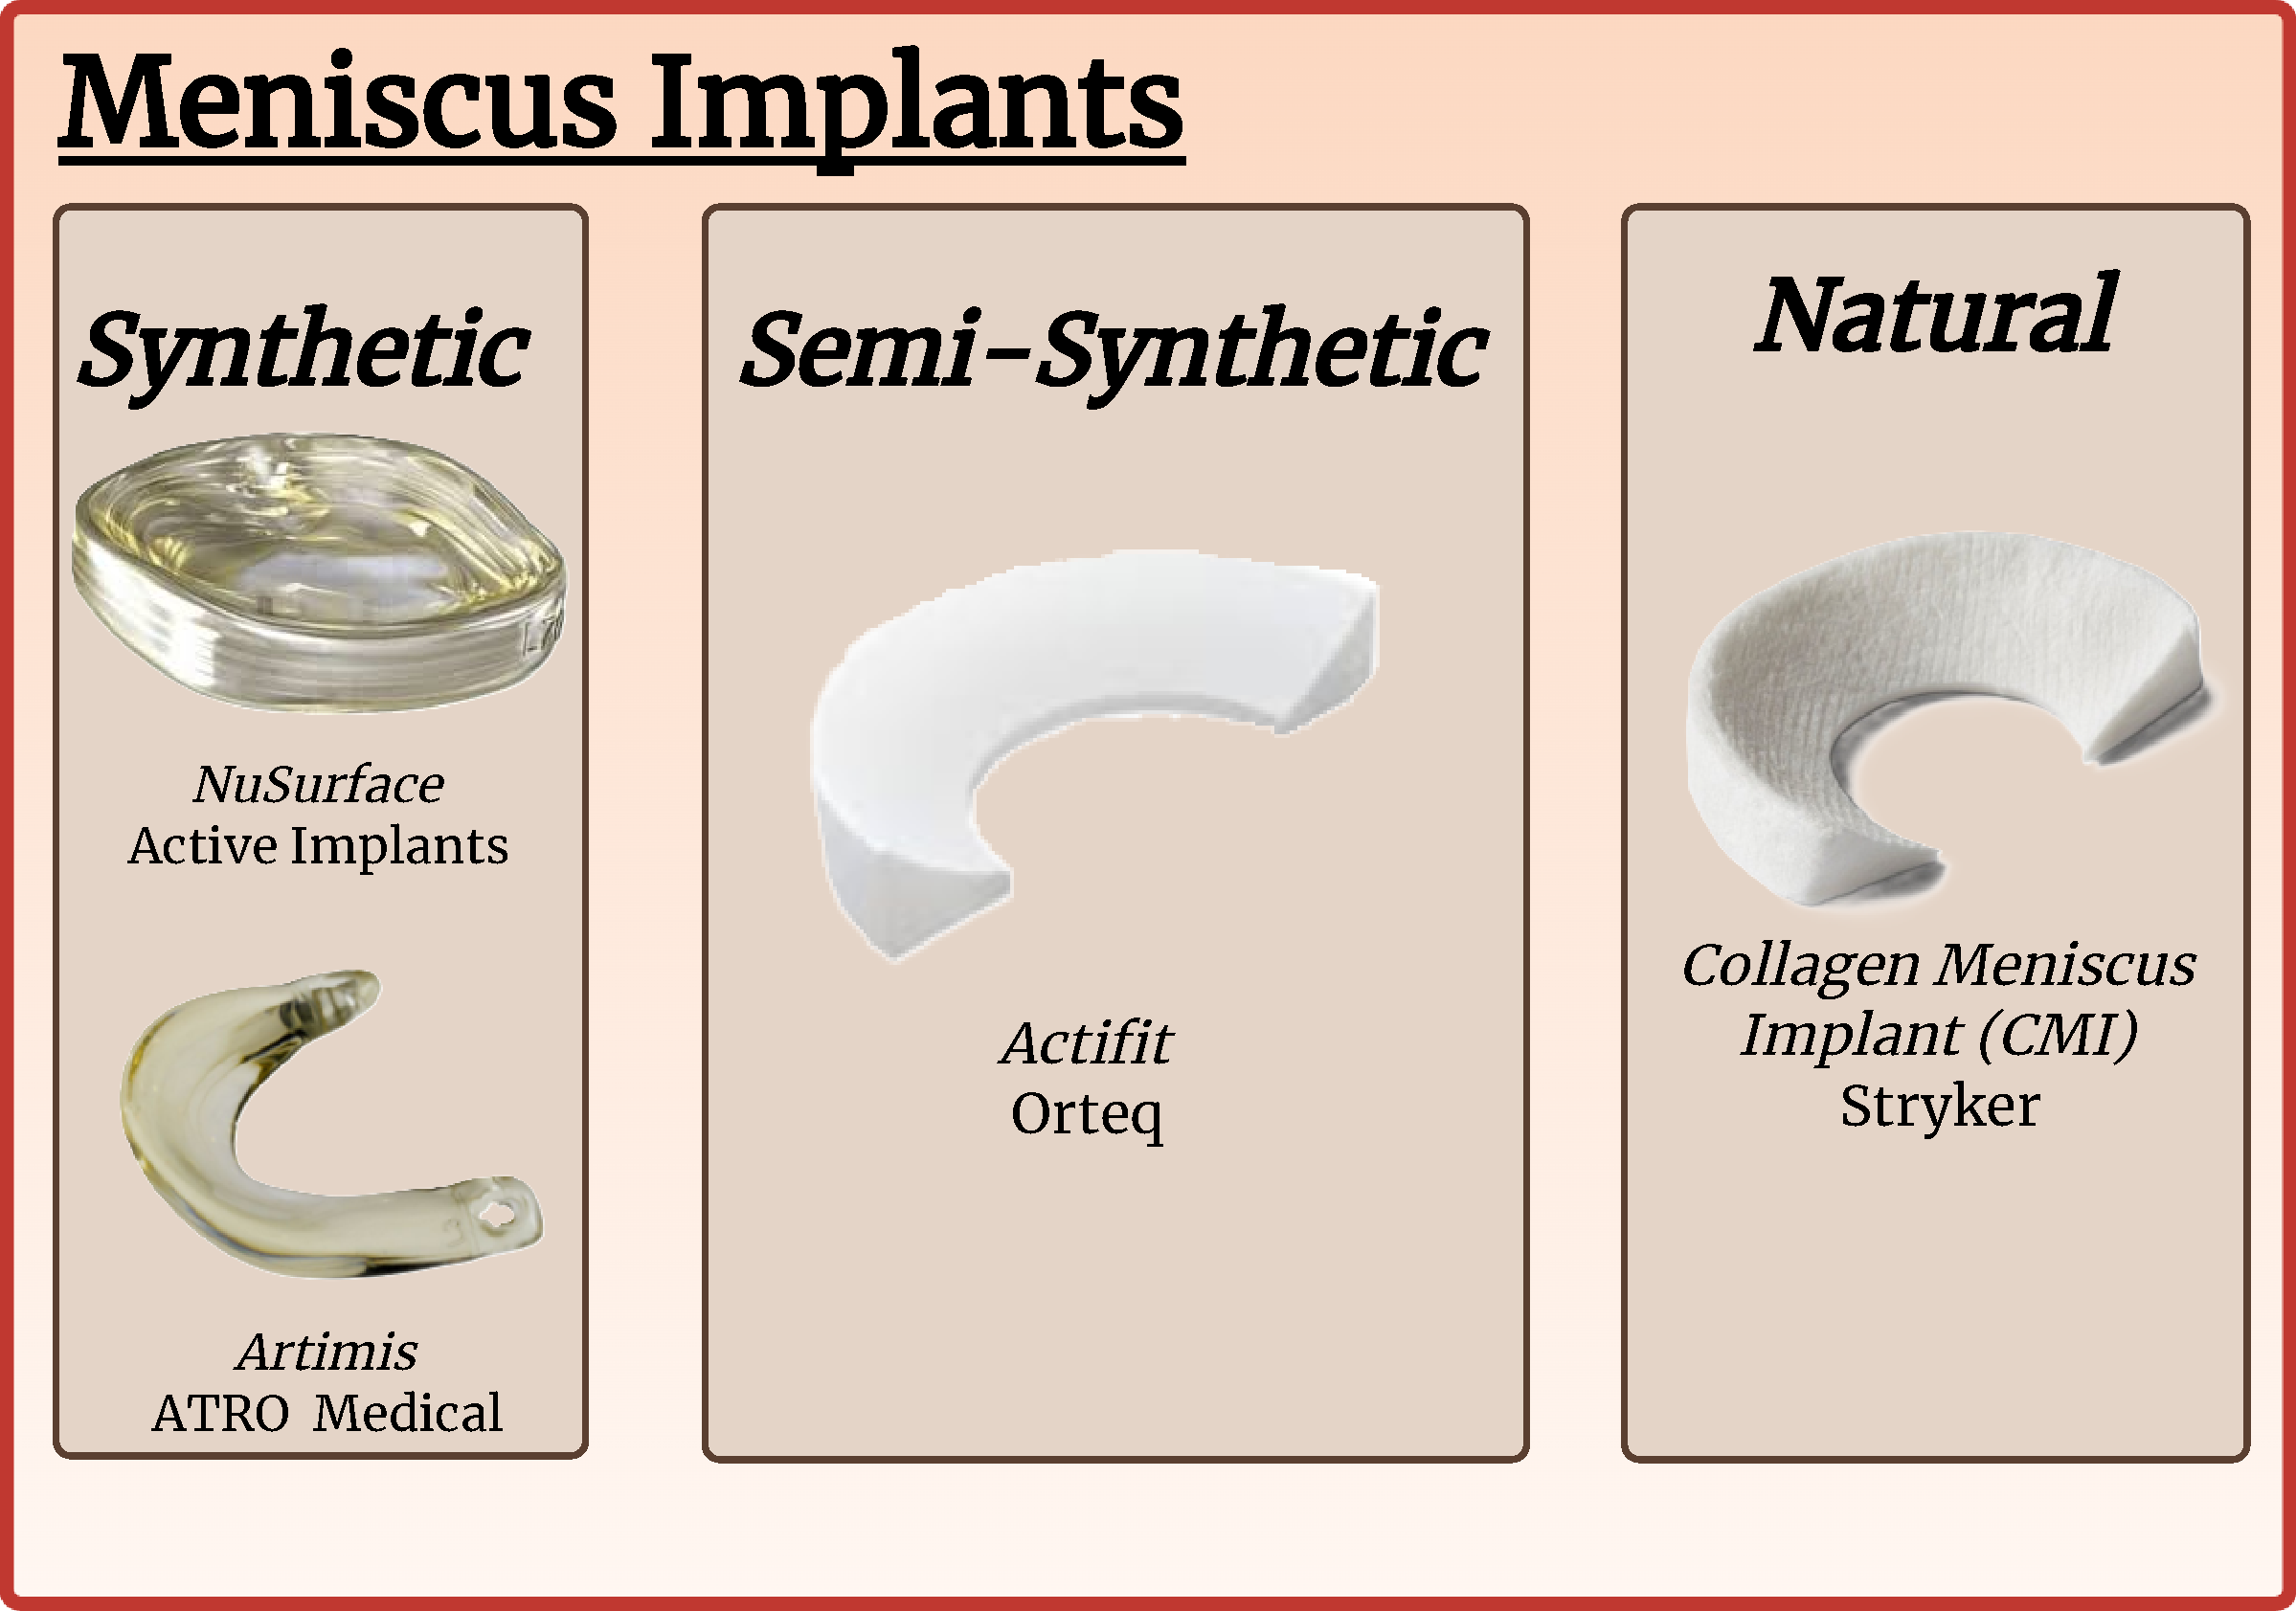
\includegraphics[width=0.85\textwidth]{figures/intro/ch1_meniscusimplants.pdf}
    \caption[Current Meniscal Implant Types]{\textbf{Current Meniscal Implant Types.} Current commercially available meniscus implants categorized by material composition. 
    \textbf{Synthetic} implants, such as the \textit{NuSurface} (Active Implants) and \textit{Artimis} (ATRO Medical), are composed of polymeric materials designed to replace mechanical function. 
    \textbf{Semi-synthetic} options, such as the \textit{Actifit} scaffold (Orteq), combine synthetic polymers with biological integration strategies.
    \textbf{Natural} scaffolds, such as the \textit{Collagen Meniscus Implant (CMI)} by Stryker, are derived from biologically based materials and aim to promote tissue regeneration.}
    \label{fig:ch1_meniscusimplants}
\end{figure}



\section{Knee Anatomy, Biomechanics, and \protect\\ Meniscal Structure}

\begin{figure}[H]
    \centering
    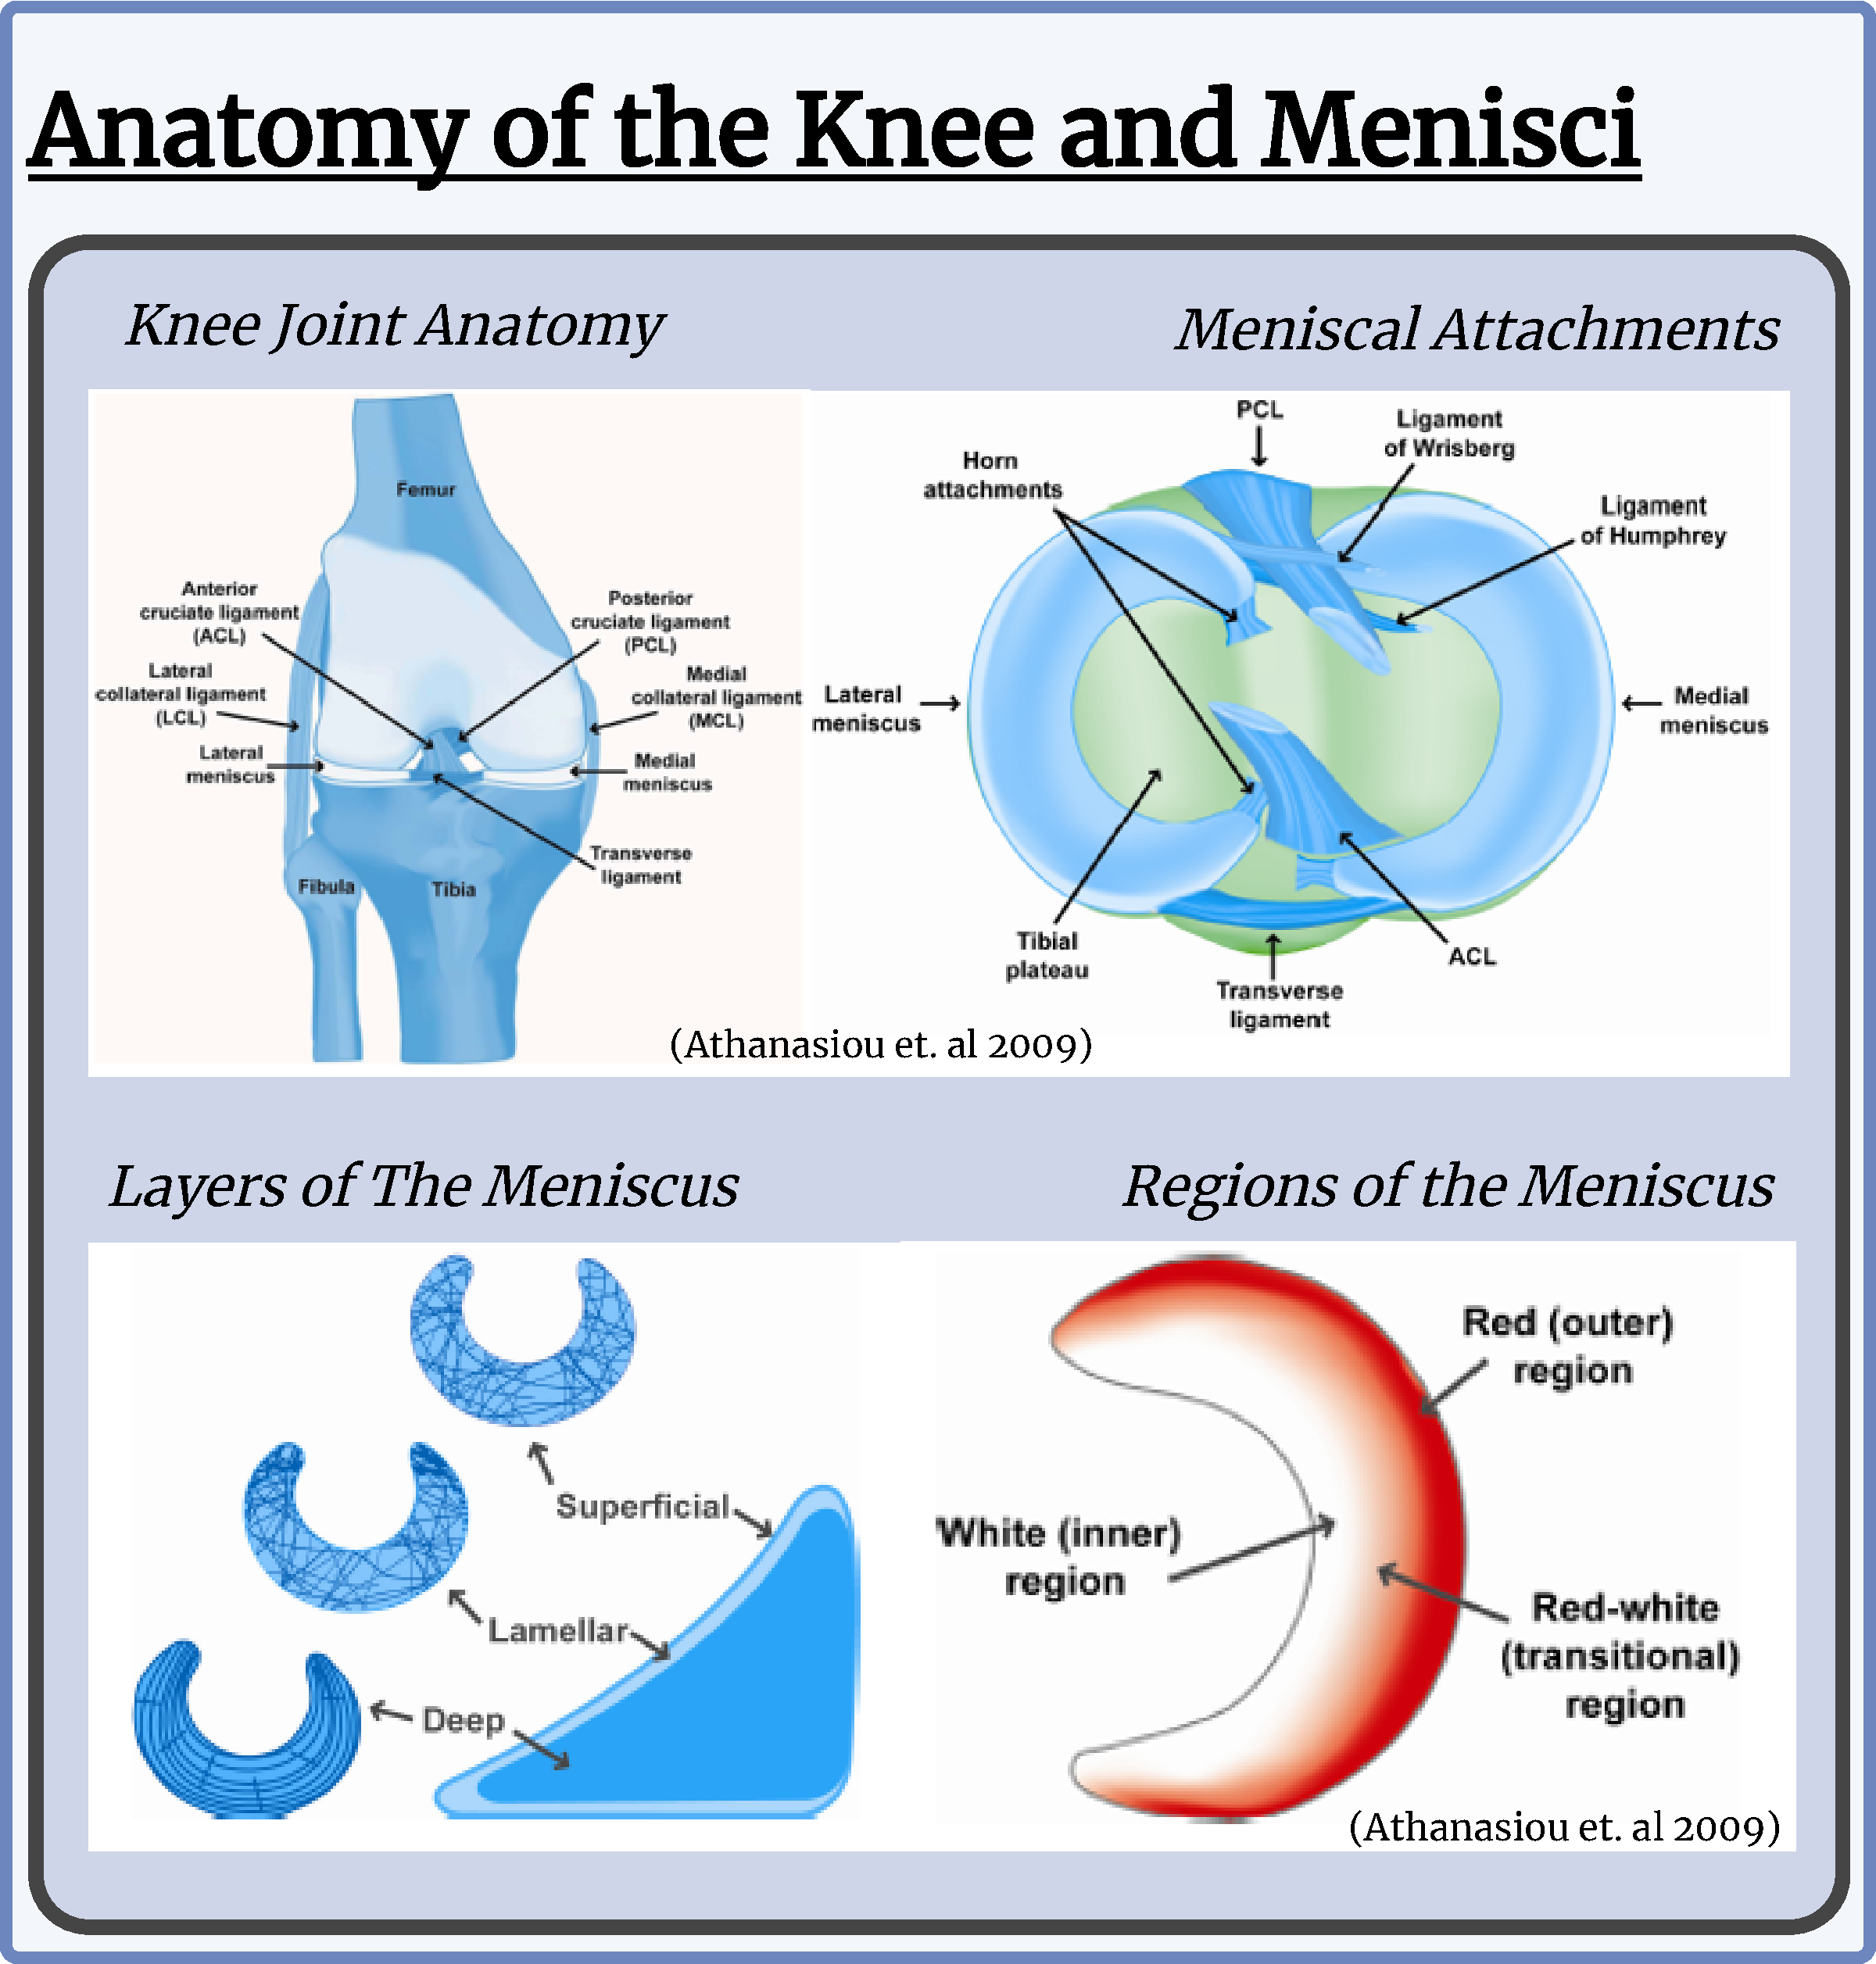
\includegraphics[width=0.9\textwidth]{figures/intro/ch1_kneeanatomy.pdf}
    \caption[Knee and Meniscal Anatomy]{\textbf{Knee and Meniscal Anatomy.} Anatomy of the Knee and Menisci. The figure highlights the major ligaments and attachments stabilizing the knee joint, as well as the layered and regional structure of the meniscus. (Adapted from \cite{athanasiou2009engineeringknee, makris2011kneemeniscus, baek2015meniscustissue})}
    \label{fig:ch1_kneeanatomy}\end{figure}

\newpage
\subsection{Knee Anatomy and Meniscal Structure}

The knee joint is a complex, load-bearing hinge joint critical for weight transmission and locomotion~\cite{makris2011kneemeniscus, athanasiou2009engineeringknee, abdelgaied2015comparisonbiomechanical}. As shown in Figure~\ref{fig:ch1_kneeanatomy}, it is formed by the articulation of the femur, tibia, and patella, stabilized by ligaments including the ACL, PCL, MCL, and LCL~\cite{athanasiou2009engineeringknee, makris2011kneemeniscus}. The menisci—medial and lateral—serve vital biomechanical functions as crescent-shaped fibrocartilaginous tissues situated between the femoral condyles and tibial plateau, providing joint congruency, load distribution, shock absorption, and friction reduction~\cite{makris2011kneemeniscus, athanasiou2009engineeringknee, baek2015meniscustissue, abdelgaied2015comparisonbiomechanical}.

Each meniscus is anchored to the tibial plateau through horn attachments and connected via ligamentous structures~\cite{athanasiou2009engineeringknee, makris2011kneemeniscus}. Vascularization is confined to the peripheral red-zone, while the central white-zone remains avascular, affecting healing potential~\cite{athanasiou2009engineeringknee, makris2011kneemeniscus, tran2020comprehensivereview}. The menisci display a highly organized internal structure with three distinct layers: superficial, lamellar, and deep~\cite{athanasiou2009engineeringknee, makris2011kneemeniscus, baek2015meniscustissue}. Each layer varies in collagen fiber orientation and mechanical function, contributing to anisotropic mechanical behavior~\cite{makris2011kneemeniscus, baek2015meniscustissue, abdelgaied2015comparisonbiomechanical}. Regional differences between red (outer), red-white (transitional), and white (inner) zones define the meniscus's response to mechanical stresses~\cite{athanasiou2009engineeringknee, makris2011kneemeniscus, baek2015meniscustissue}.

The meniscus exhibits characteristic C-shaped geometry that optimizes compressive load distribution across the tibiofemoral joint~\cite{makris2011kneemeniscus, athanasiou2009engineeringknee, baek2015meniscustissue}. This geometry increases contact area between femur and tibia, reducing peak stresses on articular cartilage~\cite{makris2011kneemeniscus, abdelgaied2015comparisonbiomechanical, baek2015meniscustissue}. The medial meniscus is more semicircular, while the lateral meniscus displays tighter curvature, contributing to functional differences in load transmission~\cite{makris2011kneemeniscus, athanasiou2009engineeringknee, baek2015meniscustissue}.

At the microscale, the meniscus possesses a hierarchical structure composed primarily of collagen fibers with proteoglycans~\cite{makris2011kneemeniscus, athanasiou2009engineeringknee, baek2015meniscustissue, abdelgaied2015comparisonbiomechanical}. Collagen fibers are anisotropically aligned across tissue zones to fulfill specialized mechanical roles~\cite{makris2011kneemeniscus, baek2015meniscustissue, abdelgaied2015comparisonbiomechanical}. The superficial layer features randomly oriented fibers for shear resistance~\cite{makris2011kneemeniscus, baek2015meniscustissue}. The lamellar layer exhibits circumferential fiber alignment supporting hoop stress resistance~\cite{makris2011kneemeniscus, baek2015meniscustissue}. The deep layer contains densely packed circumferential collagen bundles critical for withstanding tensile forces during axial compression~\cite{makris2011kneemeniscus, baek2015meniscustissue, abdelgaied2015comparisonbiomechanical}. This multiscale organization enables the meniscus to absorb dynamic loads while preserving joint stability~\cite{makris2011kneemeniscus, athanasiou2009engineeringknee, baek2015meniscustissue, abdelgaied2015comparisonbiomechanical}.

\begin{table}[H]
\centering
\setlength{\tabcolsep}{8pt}
\begin{tabular}{|l|p{5cm}|p{5cm}|}
\hline
\rowcolor{gray!20}
\textbf{Layer} & \textbf{Fiber Orientation}& \textbf{Functional Role} \\ \hline
\textbf{Superficial Layer} & Random collagen fibers on femoral and tibial surfaces & Smooth articulation, shear resistance, interface with cartilage \\ \hline
\textbf{Lamellar Layer} & Interdigitated radial and oblique fibers in the intermediate zone & Transfers loads to the core, provides structural transition \\ \hline
\textbf{Deep Layer (Core)} & Densely packed circumferential fibers with radial ties & Primary load-bearing, resists hoop stresses, maintains integrity \\ \hline
\end{tabular}
\caption[Meniscal Tissue Structure]{\textbf{Meniscal Tissue Structure.} Table summarizing the structural organization and functional roles of the distinct layers within meniscal tissue, highlighting key differences in collagen orientation and biomechanical function. Adapted from (Athanasiou et al., 2009).}
\label{tab:meniscal_structure}\end{table}

\newpage
\subsection{Tissue Composition and Biochemical Properties}

The functional capacity of the meniscus stems from its unique biochemical composition, which consists primarily of water (~70\% of total weight) and collagen (~75\% of dry weight), with additional components including glycosaminoglycans (GAGs), DNA, and minor proteins. As detailed in Table~\ref{tab:meniscus_composition}, water is crucial for the tissue's viscoelastic behavior under dynamic loading conditions, while collagen provides the essential structural framework for mechanical integrity\cite{makris2011kneemeniscus,gupta2020meniscaltissue,moutos2007biomimeticthreedimensional}.

The distribution and organization of specific components vary significantly by region within the meniscus. Type I collagen dominates the outer (red) region (90-99\% of collagen content), while the inner (white) region contains higher proportions of type II collagen to support compressive loads\cite{athanasiou2009engineeringknee,bahcecioglu20193dprinted}. Though present in smaller quantities (~1-2\% of dry weight), GAGs play a vital role in maintaining tissue hydration and resisting compression through their highly charged nature, while minor components like DNA and elastin fibers contribute to cellular function and mechanical resilience\cite{vetri2019advancedmicroscopy}.

The hydraulic permeability of meniscal tissue, which governs fluid flow and pressure distribution within the extracellular matrix, is a critical determinant of its mechanical behavior~\cite{kleinhans2018hydraulicpermeability}. This permeability varies regionally and is influenced by the tissue's composition, particularly the GAG content and collagen fiber organization. Understanding these permeability characteristics is essential for developing tissue engineering strategies that can replicate the native tissue's fluid-solid interactions and load-bearing capacity. Furthermore, the biomechanical relationship between meniscal and articular cartilage tissues reveals important insights into joint function and degeneration mechanisms~\cite{mansourbiomechanicscartilage}, highlighting how changes in meniscal properties can directly impact cartilage health and overall joint biomechanics.

This specialized biochemical composition enables the meniscus to maintain its structural integrity while adapting to the complex mechanical demands of the knee joint. The precise balance of these components, particularly the regional variations in collagen types and GAG content, allows the tissue to effectively distribute loads and maintain joint stability during both static and dynamic activities\cite{makris2011kneemeniscus,vetri2019advancedmicroscopy}.

\begin{table}[H]
    \centering
    \setlength{\tabcolsep}{8pt}
    \begin{tabular}{|p{3.2cm}|p{2.5cm}|p{6.5cm}|}
    \hline
    \rowcolor{gray!20}
    \textbf{Component} & \textbf{Percentage} & \textbf{Key Function or Details} \\ \hline
    Water & 70--80\% (wet weight) & Major contributor to viscoelastic behavior; supports fluid pressurization \\ \hline
    \multicolumn{3}{|c|}{\textbf{Dry Weight Composition}} \\ \hline
    Total Dry Weight & 20--30\% (relative to wet weight) & Reflects total mass of solid matrix components after water removal \\ \hline
    Collagen & 60--75\% of dry weight & Primary structural protein; Type I dominant in outer regions, Type II more prevalent in inner zones \\ \hline
    Glycosaminoglycans (GAGs) & 1--2\% of dry weight & Provides compressive stiffness and retains water through osmotic swelling \\ \hline
    DNA (Cellular Content) & $\sim$2\% of dry weight & Represents cellular content within the extracellular matrix \\ \hline
    Minor Proteins & $<$2\% of dry weight & Includes adhesion molecules and elastin fibers; support mechanical and cellular functions \\ \hline
    \end{tabular}
    \caption[Meniscal Tissue Composition]{\textbf{Meniscal Tissue Composition.} Biochemical composition of the meniscal tissue, distinguishing between wet and dry weight contributions, and the functional significance of each component. Adapted from Athanasiou et al. (2009).}
    \label{tab:meniscus_composition}
\end{table}

\clearpage
\subsection{Mechanical Functions and Regional Variability}

The meniscus serves essential biomechanical functions in maintaining knee joint health~\cite{wang2022advanceselectrospun}.
It distributes compressive loads across the tibial plateau, reducing focal stress on articular cartilage and preventing degeneration~\cite{boschetti2004biomechanicalproperties}.
The tissue acts as a dynamic shock absorber during weight-bearing activities~\cite{du2023meniscusheterogeneity}, while its semicircular geometry and organized fiber structure enable conformity to femoral condyles for joint stabilization~\cite{merriam2015successfultotal}.
Through its collagen network, the meniscus converts axial compression into circumferential tensile (hoop) stresses, maintaining joint congruity~\cite{bahceciogluanatomicalmeniscus, morejon2020compressiveproperties}.

These functions depend on the tissue's sophisticated mechanical properties, which derive from its structure and composition~\cite{bahcecioglu20193dprinted, vetri2019advancedmicroscopy}.
The meniscus exhibits directional anisotropy due to circumferential collagen alignment~\cite{seitz2013stressrelaxationresponse, guo20213dprintedcellfree} and viscoelastic behavior that enables adaptation to both static and dynamic forces~\cite{seitz2013stressrelaxationresponse}.
Its compressive stiffness increases with strain rate, allowing resistance to sudden impacts~\cite{wanganalysiseects, boschetti2004biomechanicalproperties, busby2013confinedcompression}.
The outer (red) zone contains dense type I collagen and is stiffer, while the inner (white) zone is more cartilage-like with higher proteoglycan and type II collagen content~\cite{bahcecioglu20193dprinted}.

Recent advances in poroelastic characterization have revealed the complex fluid-solid interactions within meniscal tissue~\cite{barsimantov2024poroelasticcharacterization}, demonstrating how hydraulic permeability and fluid pressurization contribute to the tissue's load-bearing capacity and energy dissipation mechanisms. These poroelastic properties are particularly important for understanding the meniscus's ability to distribute loads and maintain joint stability under dynamic loading conditions. The mechanical behavior of the meniscus, illustrated in Figure~\ref{fig:ch1_injuriesandmechanics}, demonstrates how axial loads are transformed into circumferential stresses through the tissue's unique architecture. This load distribution mechanism is critical for joint stability and cartilage protection.

\begin{figure}[H]
    \centering
    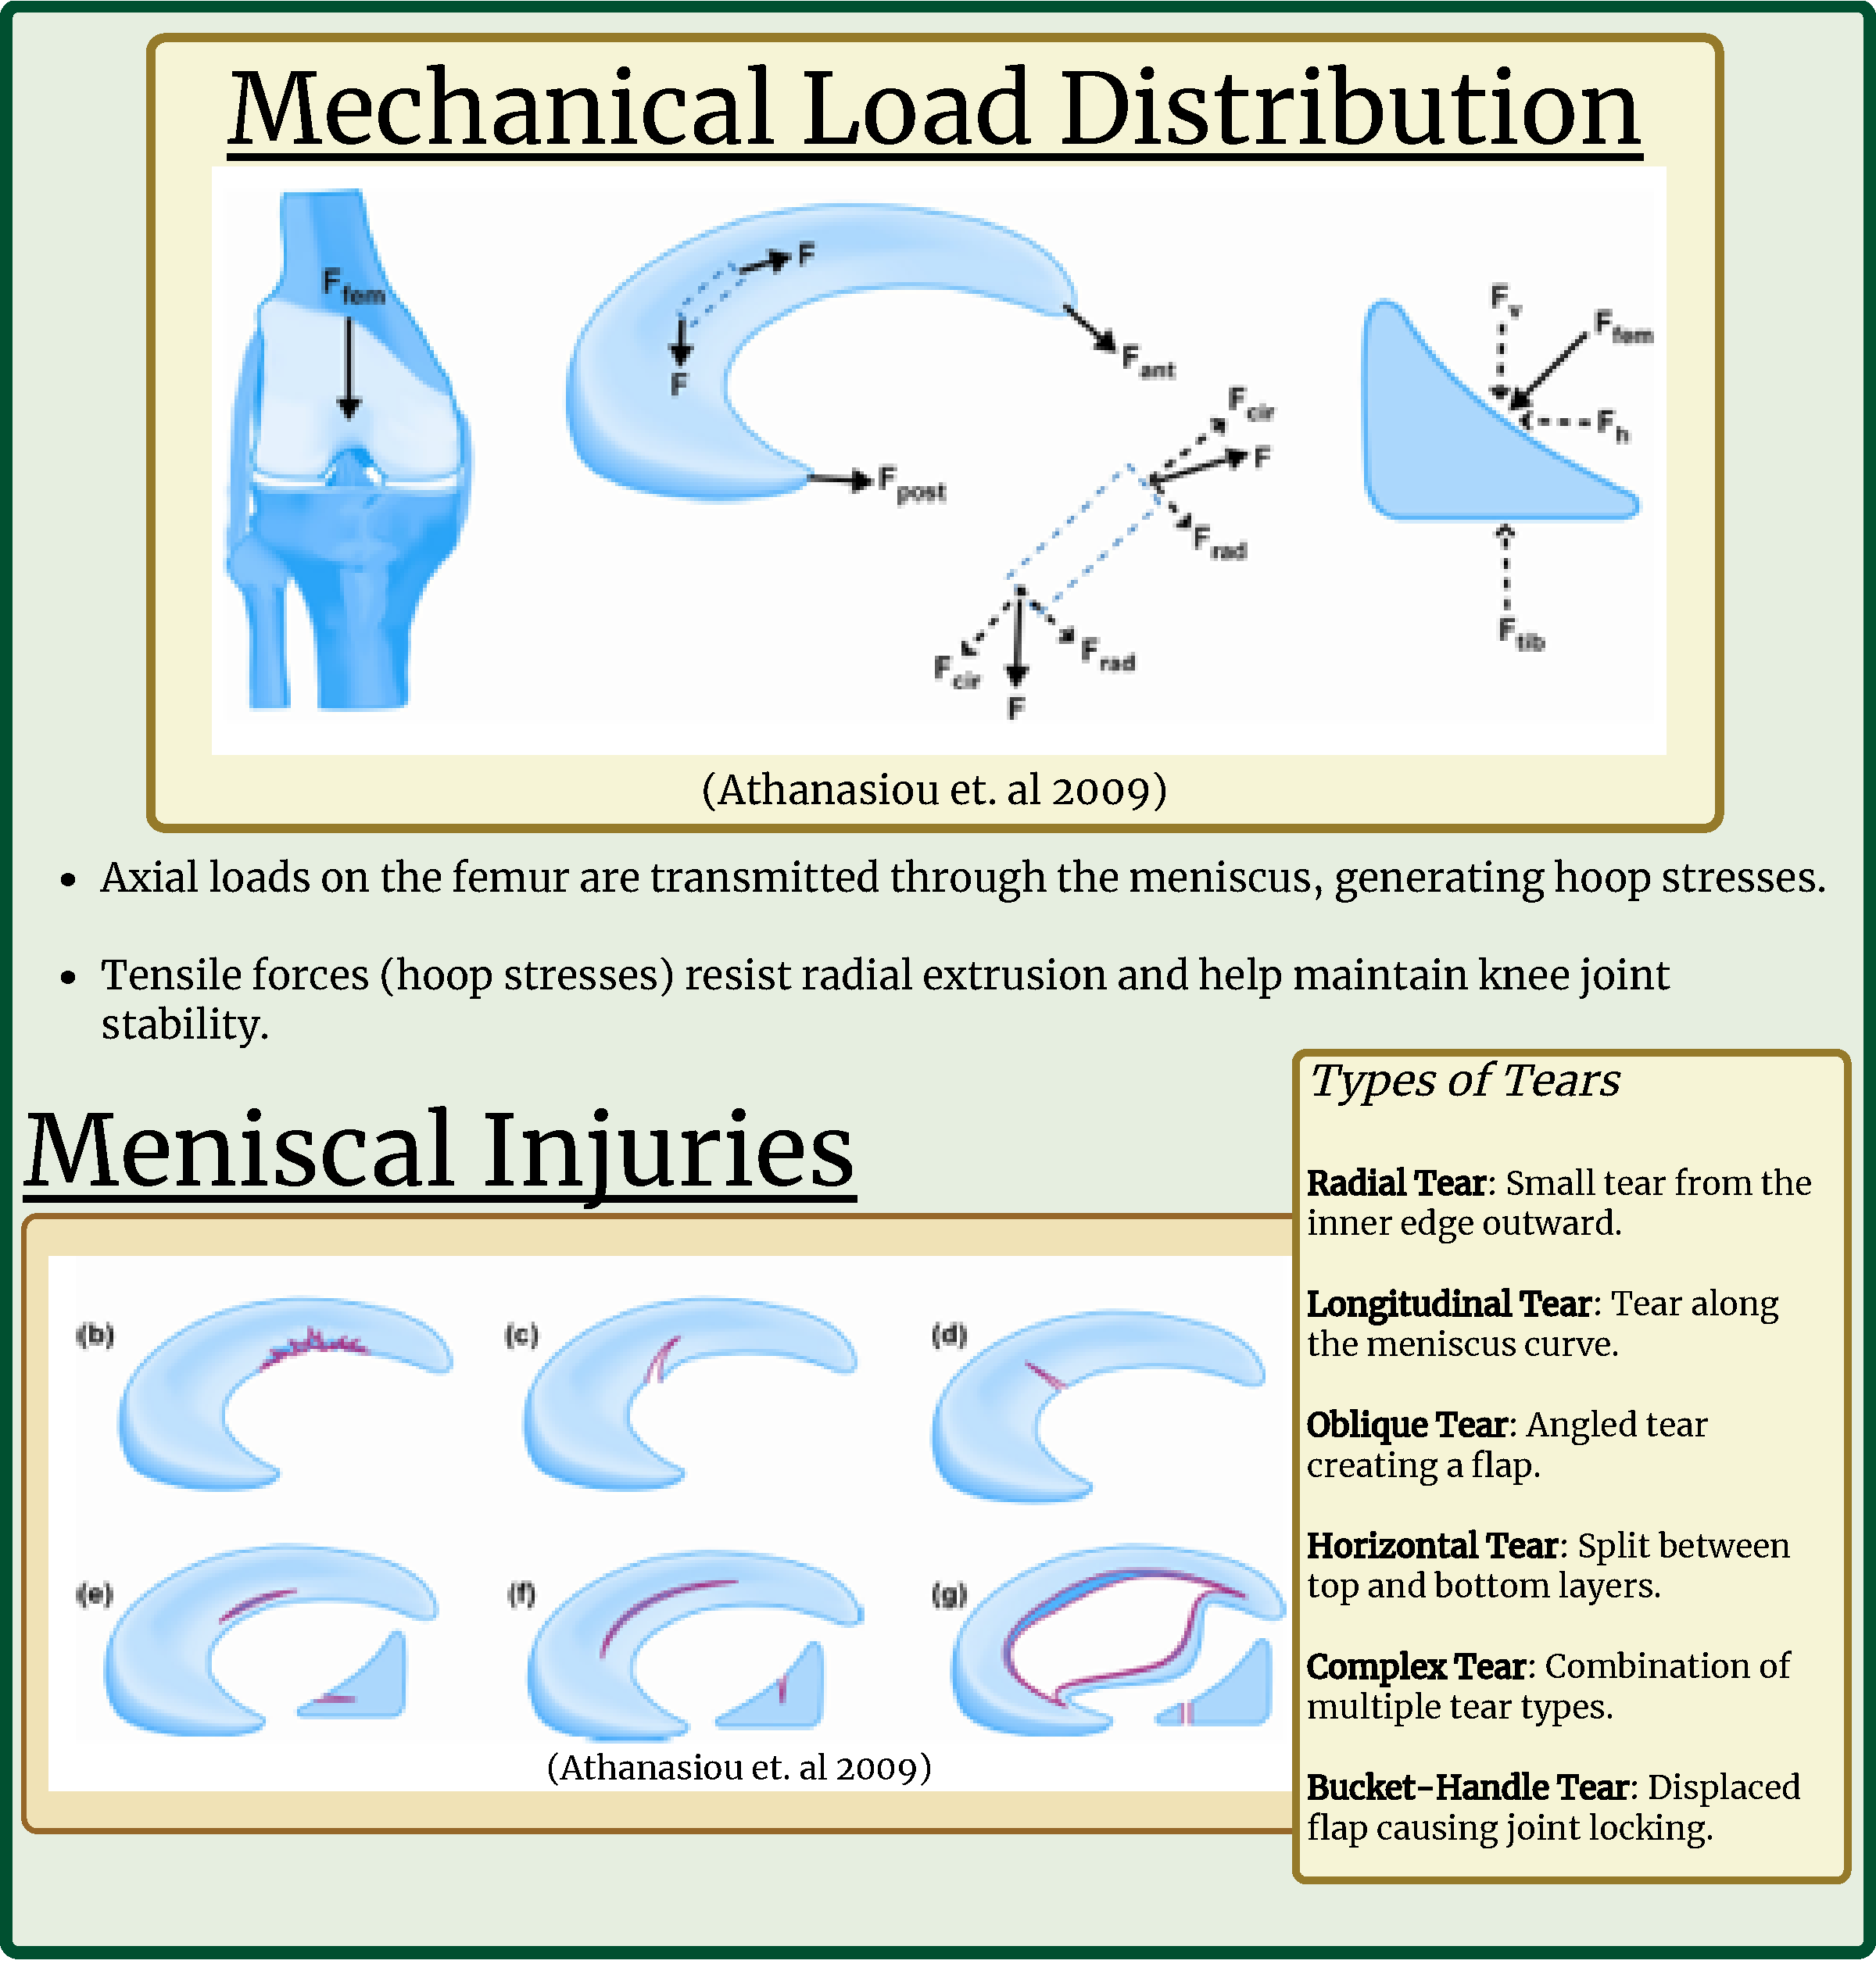
\includegraphics[width=0.85\textwidth]{figures/intro/ch1_injuriesandmechanics.pdf}
    \caption[Meniscal Load Distribution and Injury Patterns]{\textbf{Meniscal Load Distribution and Injury Patterns.} Mechanical load distribution and common meniscal injury patterns. 
    (Top) Axial loads applied to the femur are transmitted through the menisci, generating hoop stresses that resist radial extrusion and enhance joint stability. 
    (Bottom) Representative tear patterns of the meniscus, including radial, longitudinal, oblique, horizontal, complex, and bucket-handle tears, each influencing the tissue's mechanical integrity and healing capacity.(Adapted from \cite{athanasiou2009engineeringknee})}
    \label{fig:ch1_injuriesandmechanics}
\end{figure}

\section{Current Tissue Engineering \protect\\ Approaches and Limitations}

\begin{figure}[H]
    \centering
    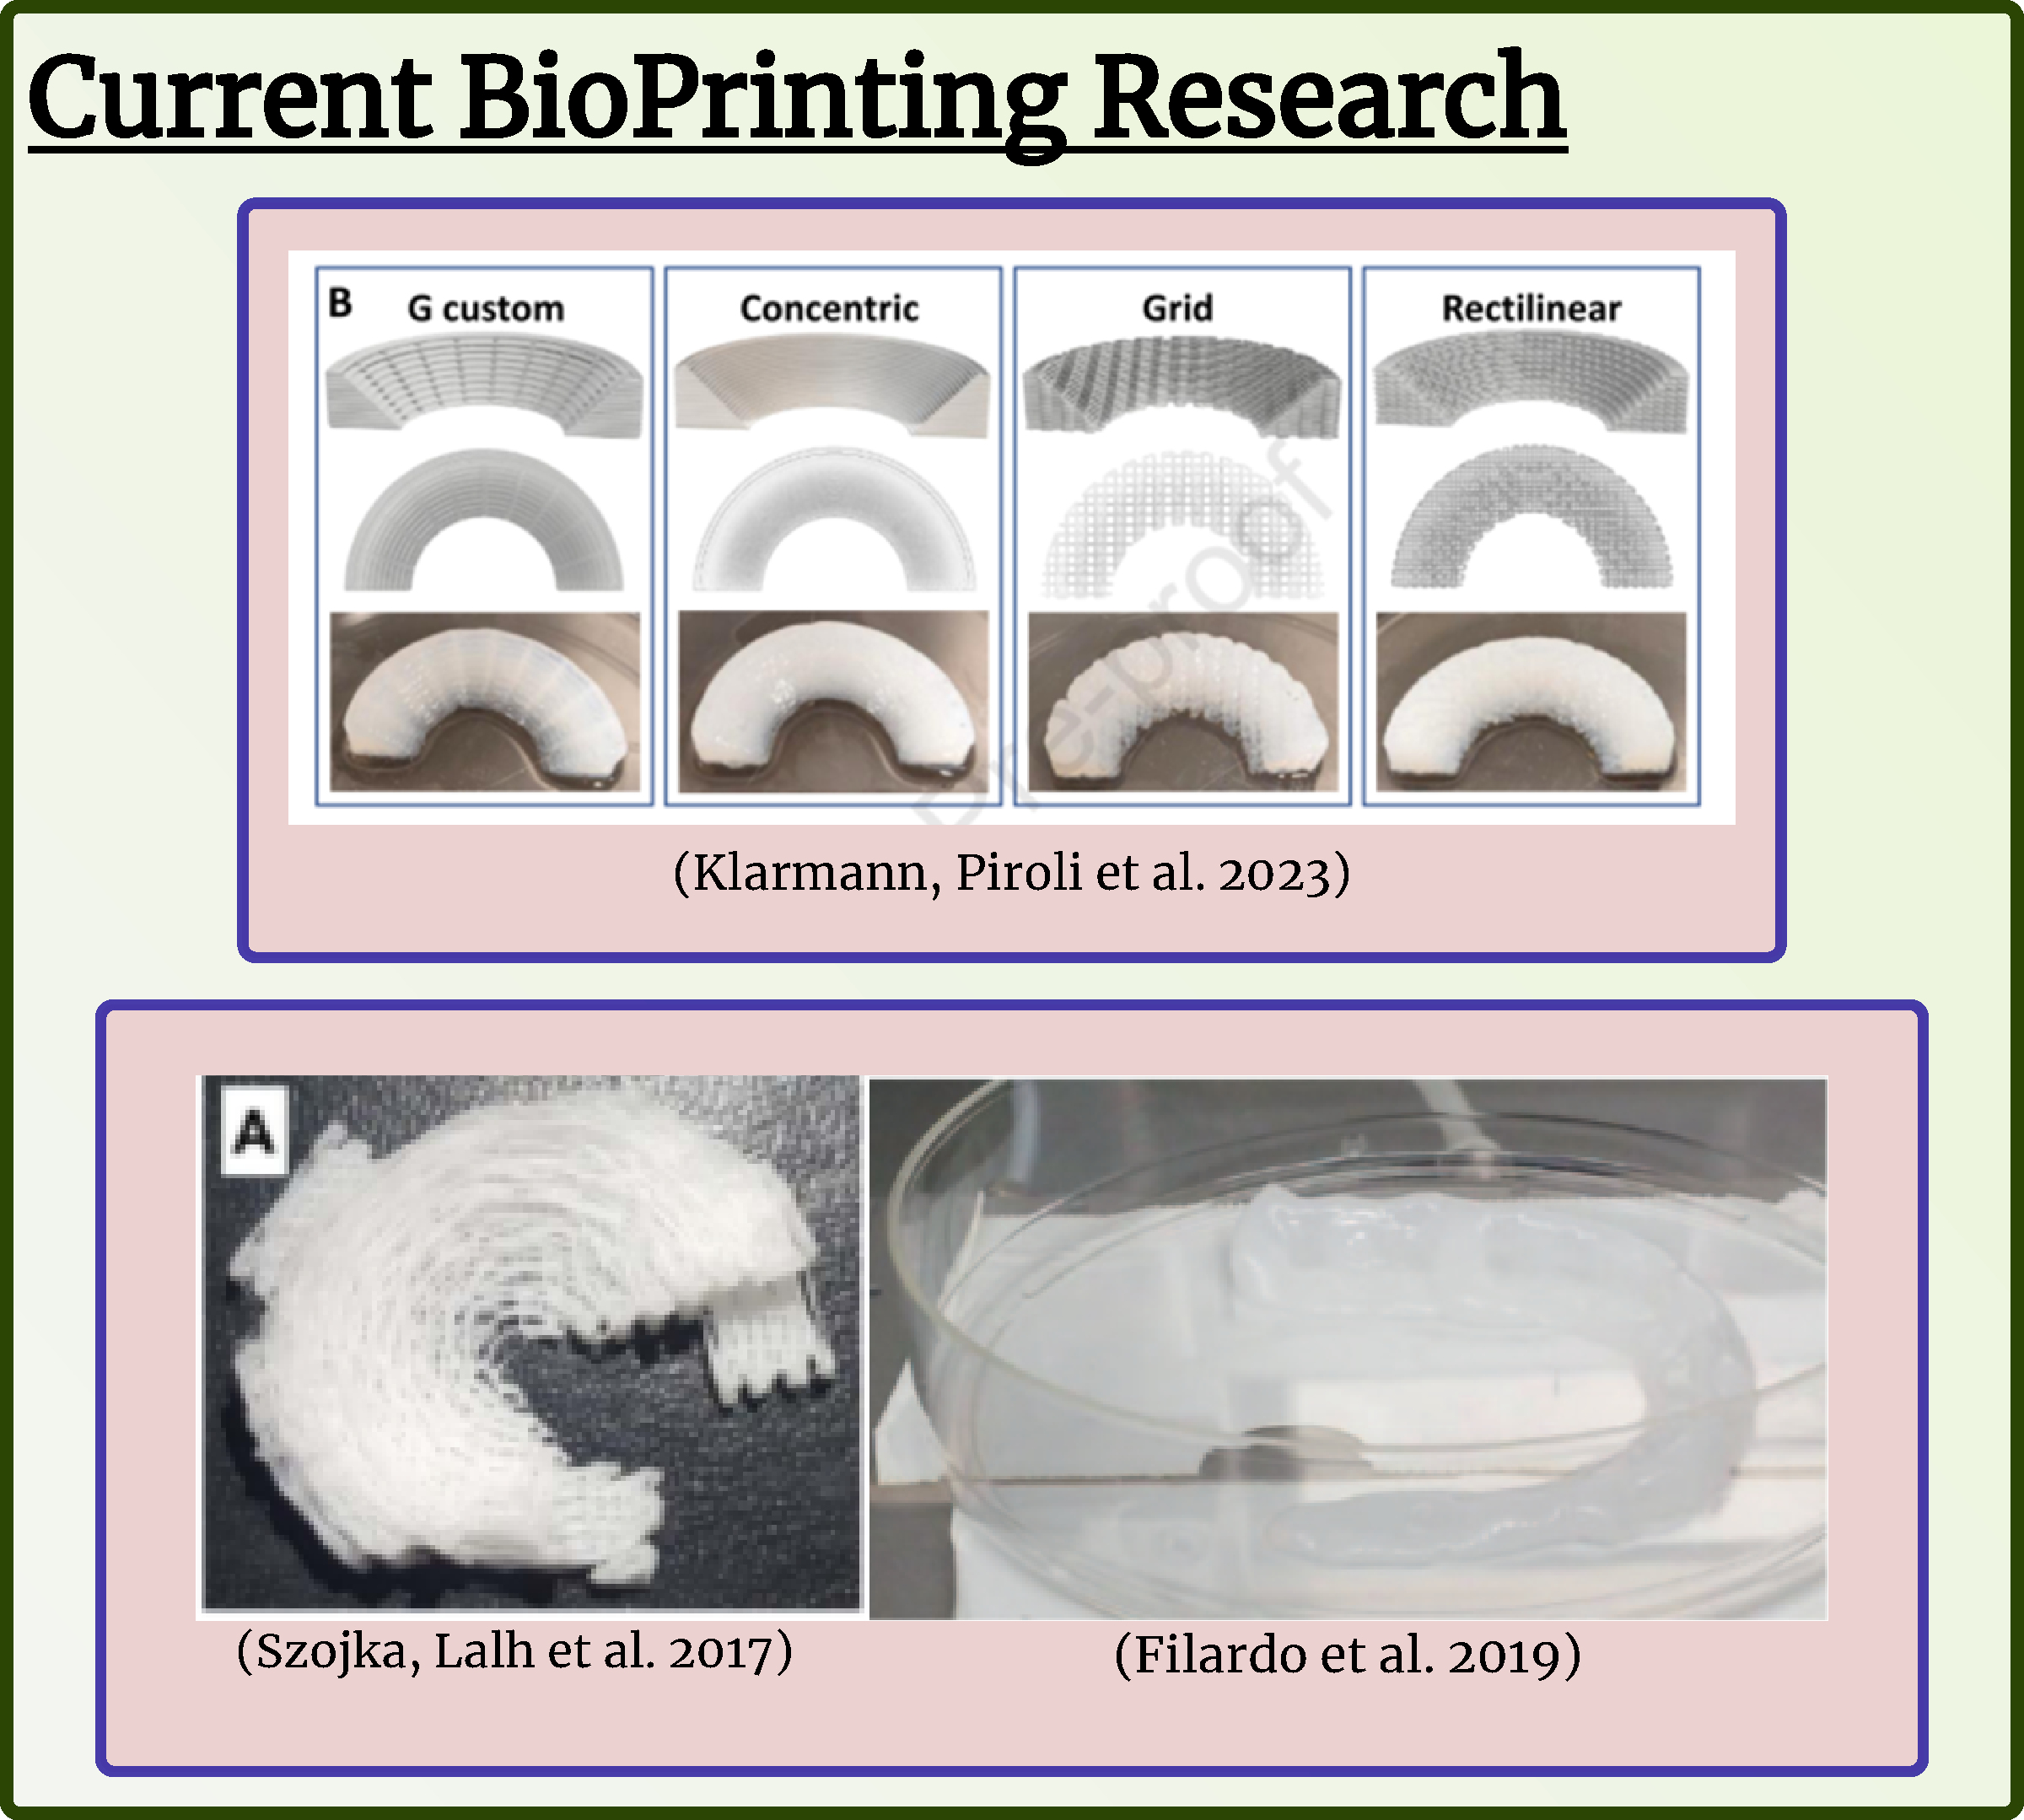
\includegraphics[width=0.85\textwidth]{figures/intro/ch1_bioprinting.pdf}
    \caption[Bioprinting Research in Meniscal Engineering]{\textbf{Bioprinting Research in Meniscal Engineering.} Examples of current bioprinting research in meniscal tissue engineering. 
    Top row: Different printing architectures (custom G-code, concentric, grid, and rectilinear patterns) for meniscal scaffold fabrication (Klarmann, Piroli et al., 2023). 
    Bottom left: Layered scaffold structure mimicking meniscal fiber orientation (Szojka, Lalh et al., 2017). 
    Bottom right: Hydrogel-based meniscus-shaped construct developed for potential tissue integration and regeneration (Filardo et al., 2019).}
    \label{fig:ch1_bioprinting}\end{figure}


\newpage
\subsection{Advances in Bioprinting for Meniscal Repair}
Bioprinting has emerged as a promising alternative to traditional meniscal repair methods, offering precise control over the spatial organization of cells, biomaterials, and bioactive signals \cite{engberg2021opensource}. This enables the fabrication of scaffolds that can mimic the native tissue's complex features including zonal organization, mechanical anisotropy, and biological complexity~\cite{sun20213dbioprintingreadytoimplant}.

Recent advances in bioprinting technologies have significantly expanded the capabilities for creating complex tissue architectures~\cite{bercea2024recent}, with particular emphasis on achieving structural fidelity that matches native tissue organization. The structural outline of meniscal tissue engineering approaches has evolved to incorporate both top-down and bottom-up fabrication strategies~\cite{brand2001structuraloutline}, enabling the creation of scaffolds with hierarchical organization that can better replicate the native tissue's mechanical and biological properties.

Current research focuses on developing bioinks from natural hydrogels, synthetic polymers, and composite materials~\cite{bahcecioglu20193dprinted, baek2015meniscustissue, a.murphy20243dprintedvariable}. These are printed in controlled architectures to recreate the regional variations in fiber orientation, stiffness, and cellular composition of native meniscus~\cite{a.murphy20243dprintedvariable, bahceciogluanatomicalmeniscus, sun20213dbioprintingreadytoimplant}.

\begin{itemize}
    \item \textbf{Material Selection:} Use of natural, synthetic, and hybrid bioinks designed to balance mechanical strength, biodegradability, and cellular compatibility.

    \item \textbf{Cell Incorporation:} Printing of constructs seeded with mesenchymal stem cells (MSCs), fibrochondrocytes, or other progenitor cell types to promote in situ tissue regeneration and matrix deposition.

    \item \textbf{Bioactive Molecule Delivery:} Incorporation of growth factors (e.g., TGF-\(\beta\), VEGF) within printed structures to stimulate tissue maturation, vascularization, and integration with host tissues.

    \item \textbf{Architectural Design:} Engineering of anisotropic fiber alignments and zonal gradations within the construct to mimic the circumferential, radial, and compressive properties of the native meniscus.

    \item \textbf{Mechanical Conditioning:} Application of dynamic mechanical stimulation in bioreactors to precondition constructs, enhancing matrix organization and mechanical properties before implantation.
\end{itemize}


\subsection{Current Limitations in Tissue Engineering Approaches}

Despite significant technological progress, current tissue engineering research faces several critical challenges, including:

\begin{itemize}
    \item \textbf{Limited Mechanical Robustness:} Engineered tissues often lack the mechanical strength required for load-bearing joint applications.
    
    \item \textbf{Extended Fabrication Times:} High-resolution printing of complex geometries requires significant time, limiting clinical practicality.
    
    \item \textbf{High Operational Costs:} Specialized bioprinting equipment and materials remain expensive, restricting widespread adoption.
    
    \item \textbf{Regulatory Barriers:} Complex, cell-laden constructs face intensive regulatory scrutiny, slowing clinical translation.
    
    \item \textbf{Integration Challenges:} Achieving seamless biological and mechanical integration with native joint tissues remains an unmet goal.
\end{itemize}

Nevertheless, ongoing advances in biomaterials, printing resolution, multi-material deposition, and in vitro maturation techniques continue to propel tissue engineering closer to clinical translation for functional meniscal regeneration.

\subsection{Engineering Requirements for Next-Generation Scaffolds}

The development of clinically viable meniscal scaffolds requires careful consideration of multiple design criteria that span mechanical, biological, and clinical translation domains. These requirements must be addressed simultaneously to create scaffolds that can withstand physiological loading while promoting tissue regeneration and maintaining cost-effective manufacturability. The following subsections outline the key design targets for next-generation meniscal scaffolds.

\subsection{Mechanical Performance Requirements}

Mechanical performance is one of the most critical design considerations for next-generation meniscal scaffolds~\cite{sun2017overviewscaffold, gupta2020meniscaltissue, ma2025structurallysophisticated}.
The native meniscus plays a vital role in distributing compressive loads, transforming them into circumferential tensile stresses, and maintaining overall joint stability during dynamic activities~\cite{makris2011kneemeniscus}.
Therefore, engineered scaffolds must replicate key mechanical behaviors of the meniscus, including compressive stiffness, anisotropic load-bearing capacity, viscoelastic stress relaxation, and long-term durability under cyclic physiological loading~\cite{seitz2013stressrelaxationresponse, a.murphy20243dprintedvariable, sun2017overviewscaffold}.
Achieving these properties ensures that the scaffold can protect the underlying articular cartilage, resist extrusion, and maintain structural integrity throughout the healing process\cite{patel2018tissueengineeredtotal, sun2017overviewscaffold}
Failure to match these mechanical demands not only compromises functional restoration but may also accelerate degenerative changes within the joint~\cite{ghodbane2019partialmeniscus, makris2011kneemeniscus}.

Key mechanical design targets include:

\begin{itemize}
    \item \textbf{Compressive Stiffness:} Aggregate modulus in the range of 100–150 kPa to match native meniscal compression resistance~\cite{morejon2020compressiveproperties}.
    
    \item \textbf{Anisotropic Behavior:} Ability to transform axial compressive forces into circumferential tensile hoop stresses, reflecting the fiber orientation of native tissue~\cite{makris2011kneemeniscus}.
    
    \item \textbf{Viscoelastic Properties:} Stress relaxation and creep behavior similar to native meniscus to dissipate dynamic loads effectively~\cite{mordecai2014treatmentmeniscal}.
    
    \item \textbf{Fatigue Resistance:} Structural stability under millions of cyclic loading cycles experienced during normal gait and activity.
    
    \item \textbf{Dimensional Integrity:} Maintenance of anatomical shape and load-bearing surface under physiological joint forces.
\end{itemize}

\subsection{Biological Integration Requirements}

Biological integration is essential for the long-term success of meniscal scaffolds, ensuring not only initial biocompatibility but also active participation in tissue regeneration~\cite{ma2025structurallysophisticated, li20213dprinted, li2024advancedhydrogel, luis20203ddirect, shamloo2018acceleratedfullthickness}.
Scaffolds must create a permissive environment for cellular infiltration, proliferation, and extracellular matrix deposition while minimizing inflammatory responses that could lead to fibrosis or implant failure~\cite{shamloo2018acceleratedfullthickness, xu2013hybridprinting}. Successful biological integration also requires controlled scaffold degradation synchronized with new tissue formation, allowing gradual transfer of mechanical loads to the regenerating meniscus~\cite{morenonieto2021productdesign, pitt1981aliphaticpolyesters}. Moreover, the scaffold must achieve firm biological and mechanical anchorage with the surrounding native tissues to restore functional continuity within the joint~\cite{ghodbane2019partialmeniscus}. Without robust integration, even mechanically competent constructs are unlikely to achieve durable clinical outcomes~\cite{bakerengineeringanatomicallyshaped}.

Key biological design targets include:

\begin{itemize}
    \item \textbf{Biocompatibility:} Scaffold materials must minimize immune and inflammatory responses, supporting a regenerative healing environment \cite{beeler2020meniscussizing,li2024totalmeniscus}.
    
    \item \textbf{Cellular Infiltration and Remodeling:} Scaffolds should enable cell migration, attachment, proliferation, and matrix deposition to promote functional neotissue formation\cite{gupta2020meniscaltissue,du2023meniscusheterogeneity}.
    
    \item \textbf{Host Tissue Integration:} Constructs must bond with adjacent meniscal and articular cartilage tissues to restore mechanical continuity and biological functionality \cite{li2024totalmeniscus,mauck2000functionaltissue,lopez-calzada2016developmentmeniscus,yan2023meniscalfibrocartilage}.
    
    \item \textbf{Controlled Biodegradation:} Scaffold degradation should be timed to coincide with tissue regeneration, maintaining mechanical support during early healing while allowing eventual load transfer to new tissue\cite{wang20203dprinting,choi20213dprintedgelatin}.
\end{itemize}

\subsection{Clinical Translation Requirements}

Clinical translation is a critical consideration in the design of next-generation meniscal scaffolds~\cite{sun2017overviewscaffold}.
Beyond biological and mechanical performance, scaffolds must be manufactured reproducibly and economically to facilitate widespread clinical adoption~\cite{luis20203ddirect,vila2021bioengineeredoptogenetic, xiao2013mechanicaltesting}.
Fabrication techniques must support consistent scaffold architecture, scalability for large patient populations, and compatibility with established sterilization protocols to meet regulatory and clinical standards~\cite{gupta2020meniscaltissue}. Additionally, constructs must maintain dimensional stability throughout manufacturing, storage, and implantation processes to ensure anatomical accuracy and mechanical functionality~\cite{norberg2021viscoelasticequilibrium, woodruff2010returnforgotten}. Finally, cost-effective production using accessible platforms, such as desktop-scale bioprinters, is essential to reduce healthcare costs and expand global accessibility to regenerative therapies~\cite{sooriyaarachchi2019hybridfabrication, fares2018interpenetratingnetwork, gautam2013fabricationcharacterization, elkommos2025hybridhydrogels}.

In addition to these design requirements, future clinical translation will necessitate rigorous preclinical testing and navigation of regulatory frameworks to ensure safety and efficacy.
This includes comprehensive biocompatibility assessments, mechanical validation under physiological conditions, and demonstration of long-term stability in relevant animal models.

Key clinical design targets include:

\begin{itemize}
    \item \textbf{Reproducible Fabrication:} Scaffold manufacturing processes must produce consistent structural and functional outcomes across multiple batches and sites.
    
    \item \textbf{Sterilization Compatibility:} Materials and scaffold architectures must withstand standard sterilization methods without compromising mechanical or biological properties.
    
    \item \textbf{Dimensional Stability:} Constructs must preserve anatomical geometry and mechanical integrity during processing, handling, and surgical placement \cite{makris2011kneemeniscus}.
    
    \item \textbf{Cost-Effective Manufacturing:} Scaffold production should be affordable and feasible using scalable, accessible equipment such as desktop 3D bioprinting systems \cite{bahcecioglu20193dprinted,klarmann20233dprinting,elkommos2025hybridhydrogels}.
\end{itemize}

In summary, achieving a biomimetic, mechanically robust, and biologically active scaffold remains the critical design challenge in engineering a clinically translatable meniscal replacement.
A successful scaffold must exhibit poroviscoelastic behavior, mimic the mechanical anisotropy of native meniscal tissue, support cellular activity, and maintain cost-effective manufacturability for widespread clinical application.

\newpage
\section{The HANI Platform: A Hybrid Solution}

The HANI platform represents a novel and comprehensive approach to meniscal tissue engineering, integrating recent advances in biomaterials science and additive manufacturing technologies. This section describes the fundamental rationale, key components, and significant advantages of the HANI strategy.

Meniscal repair strategies including surgical interventions, tissue engineering constructs, and additive manufacturing technologies have made significant strides but consistently fall short of replicating the complex multifunctional demands of native meniscal tissue~\cite{makris2011kneemeniscus, luis20203ddirect, ma2025structurallysophisticated}.
Surgical repairs often compromise joint biomechanics and accelerate tissue degeneration~\cite{mordecai2014treatmentmeniscal,sun20213dbioprintingreadytoimplant}.
Tissue engineered scaffolds struggle to achieve an optimal balance between mechanical strength and biological functionality, and while additive manufacturing offers unprecedented architectural precision, both scalability and clinical practicality remain major obstacles~\cite{mordecai2014treatmentmeniscal,sun20213dbioprintingreadytoimplant,li20213dprinted}.

To address these persistent challenges, a hybrid regenerative strategy is required one that combines the mechanical robustness of synthetic polymers, the biological compatibility of natural hydrogels, and scalable, cost effective fabrication methods.
The Hybrid Hydrogels Augmented via Additive Network Integration (HANI) platform was developed to meet these critical needs, offering an integrated scaffold system specifically designed to restore both mechanical resilience and biological functionality\cite{elkommos2025hybridhydrogels}.

\begin{figure}[H]
    \centering
    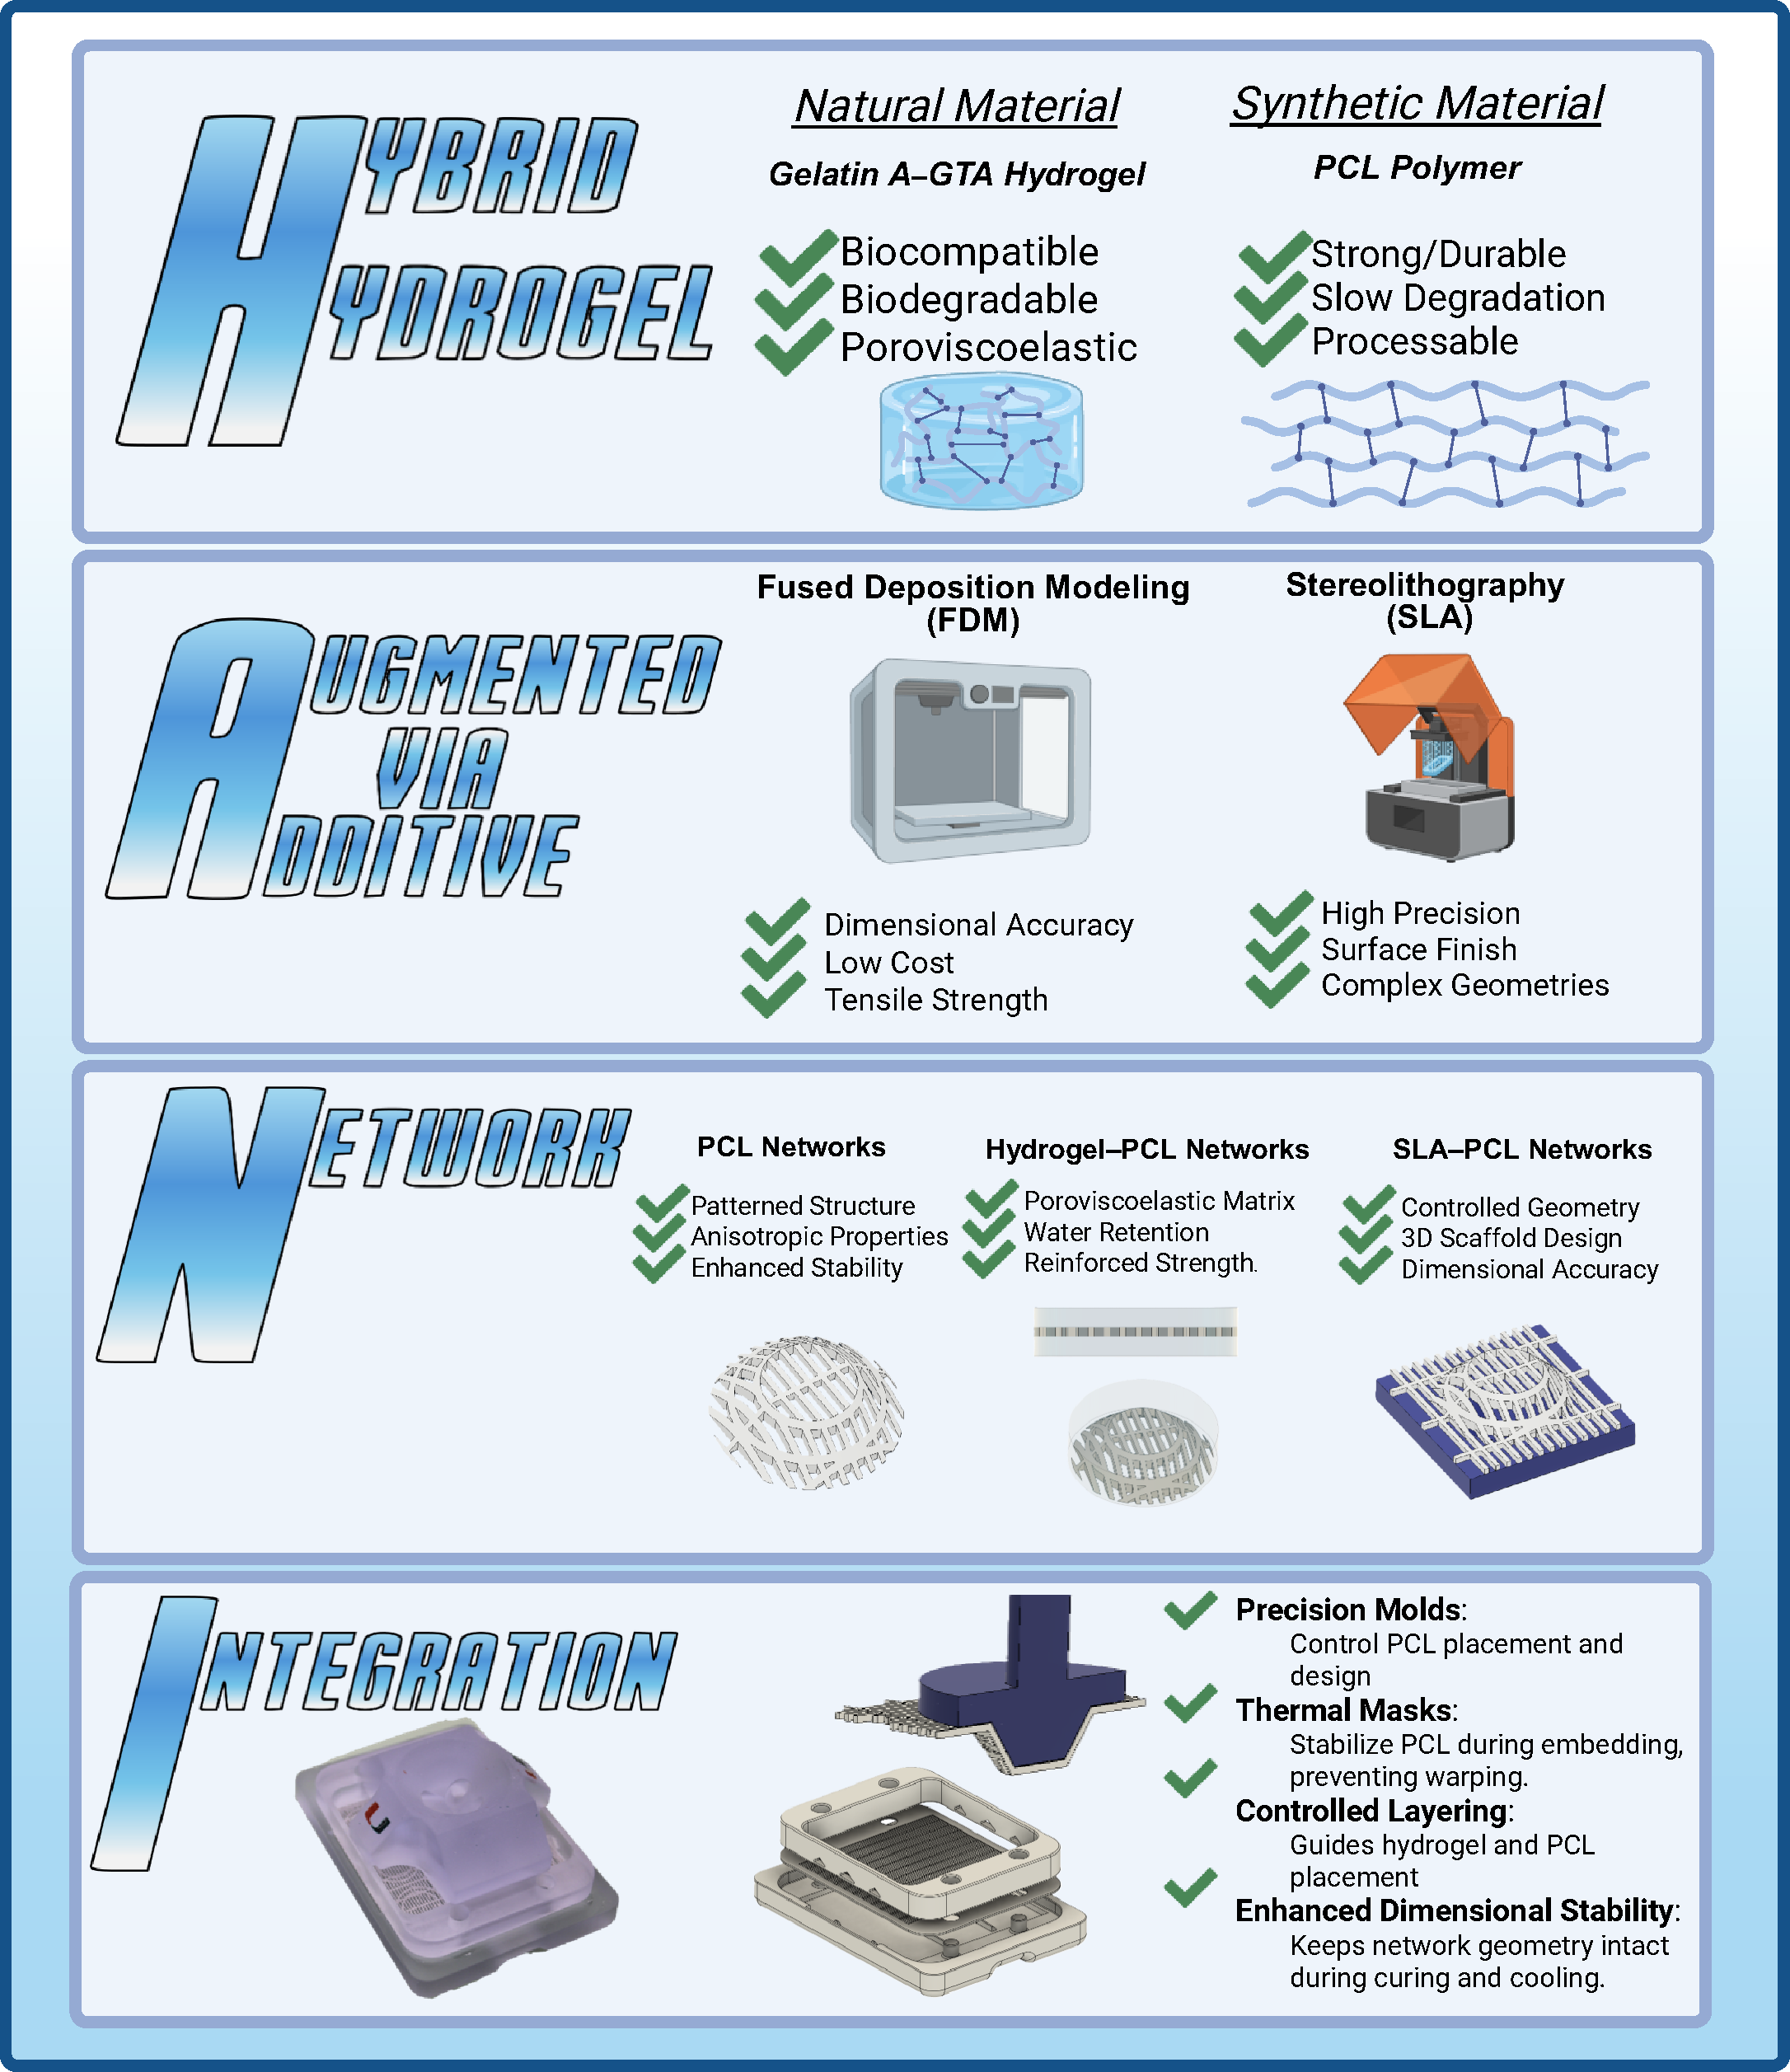
\includegraphics[width=0.85\textwidth]{figures/intro/ch1_HANI.pdf}
    \caption[HANI Platform Overview]{\textbf{HANI Platform Overview.} The HANI strategy combines natural gelatin-based hydrogels and synthetic polycaprolactone (PCL) polymers to achieve balanced biocompatibility, mechanical strength, and poroviscoelastic behavior. Additive manufacturing techniques (FDM and SLA) are utilized to fabricate precise reinforcement networks and molds. Integrated architectures and thermal stabilization ensure structural integrity during hydrogel embedding and curing, enabling scalable fabrication of robust, biologically compatible scaffolds.}
    \label{fig:ch1_HANI}
\end{figure}

\subsection{Platform Components and Design Strategy}

The HANI platform represents a strategic response to the current limitations in meniscal tissue engineering, combining advanced hydrogel chemistry, synthetic reinforcement networks, and precision additive manufacturing to engineer functionally relevant, clinically translatable meniscal replacements.
This integrated approach directly addresses the key challenges identified in current tissue engineering research while offering several distinct advantages~\cite{elkommos2025hybridhydrogels}.

By leveraging the synergistic properties of natural and synthetic materials, the HANI platform achieves mechanical robustness without compromising biological functionality, while maintaining scalable and cost-effective manufacturing processes essential for clinical translation~\cite{sun2017overviewscaffold, luis20203ddirect, bahcecioglu20193dprinted}.

The HANI platform integrates four key components:

\begin{itemize}
    \item \textbf{Hybrid Hydrogel (H):} Combines gelatin-based hydrogel (GelA) with PCL reinforcement networks and controlled crosslinking (GTA) to achieve optimal mechanical and biological properties
    \item \textbf{Augmented via Additive (A):} Utilizes Fused Deposition Modeling (FDM) and Stereolithography (SLA) for precise control over scaffold architecture and mechanical properties
    \item \textbf{Network (N):} Incorporates hydrogel-PCL networks, aligned networks for directional reinforcement, circumferential networks for hoop stress distribution, and 3D thermomolded structures
    \item \textbf{Integration (I):} Ensures structural integrity through thermal stabilization, dimensional control, and scalable fabrication processes
\end{itemize}

This integrated strategy seeks to overcome the trade-offs inherent in current meniscal engineering methods by combining mechanical performance, biological integration, and scalable manufacturing.

\subsection{Biomaterial Components and Platform Advantages}

Gelatin-based hydrogel (GelA), derived from collagen, is widely used in tissue engineering due to its intrinsic biocompatibility, biodegradability, and cell-adhesive properties. Its tunable polymer concentration and crosslinking density allow the engineering of hydrogels with physiologically relevant water content and stress-relaxation behavior, making it an ideal candidate for soft tissue scaffolds.

Poly-$\varepsilon$-caprolactone (PCL) is a synthetic, biodegradable polymer with excellent mechanical strength and flexibility \cite{cipitria2011designfabrication}. When fabricated into reinforcing networks via FDM, PCL enhances the structural integrity of GelA-based constructs and enables the creation of anisotropic load-bearing architectures, critical for mimicking the mechanical function of native meniscus.

The combination of GelA hydrogels and PCL reinforcement networks enables the fabrication of composite scaffolds that integrate biological functionality with mechanical resilience. Composite designs can be engineered to reproduce the viscoelastic, anisotropic behavior of native meniscal tissue, providing a platform for functional tissue regeneration.

The HANI platform advances meniscal tissue engineering by addressing the longstanding trade-offs between mechanical strength and biological functionality. The combined material and manufacturing approach provides:

\begin{itemize}
    \item Tunable mechanical and poroviscoelastic behavior
    \item Enhanced biological compatibility and nutrient diffusion
    \item Scalable, cost-effective fabrication for potential patient-specific applications
    \item Enhanced cellular biointegration
    \item Patient-specific manufacturing using accessible equipment
    \item Cost-effective alternatives to traditional bioprinting technologies
\end{itemize}

Together, these innovations position the HANI approach as a transformative strategy in the development of next-generation meniscal replacements.

\section{Research Objectives and Dissertation Structure}

This dissertation addresses critical gaps in meniscal tissue engineering through a systematic investigation of the Hybrid Hydrogel Augmented via Additive Network Integration (HANI) platform\cite{elkommos2025hybridhydrogels}. The research strategy is organized into a progression of interconnected studies, each building upon previous findings to develop a comprehensive solution for functional meniscal tissue replacement. The overarching goal is to create biomimetic scaffolds that replicate both the mechanical and biological properties of native meniscal tissue while maintaining clinical translatability and cost-effectiveness.

The research objectives are structured to systematically address the key challenges in meniscal tissue engineering through five interconnected chapters:

\textbf{Chapter~\ref{chap:intro}: Introduction and Background} provides a comprehensive overview of meniscal tissue engineering challenges, current solutions, and the rationale for the HANI platform. This chapter establishes the clinical context and biological foundation through literature review, gap analysis, and project objectives. The expected outcome is the establishment of the need for hybrid hydrogel and additive manufacturing approaches in addressing current treatment limitations.

\textbf{Chapter~\ref{chap:2}: Hybrid Hydrogel Development and Characterization} focuses on the development and optimization of gelatin-based hydrogel formulations with native-like water content, swelling, and tunable mechanical properties. Key methods include hydrogel characterization, swelling studies, and mechanical and stress-relaxation testing. The chapter aims to identify GelA/GTA formulations with physiologically relevant properties and demonstrate tunable stress relaxation via network design.

\textbf{Chapter~\ref{chap:3}: Augmented via Additive} addresses the development of custom instrumentation and methodologies for advanced mechanical testing of hydrogels. The research employs additive manufacturing of testing apparatus, CAD design, validation, and data acquisition techniques. The expected outcome is reliable, physiologically relevant measurement of poroviscoelastic properties essential for scaffold characterization.

\textbf{Chapter~\ref{chap:4}: Additive Network Integration} explores the design and fabrication of PCL reinforcement architectures and their integration with hydrogels. The methodology encompasses FDM printing, network design optimization, and integration protocols. This chapter aims to achieve stable, biomimetic PCL-hydrogel composites with tunable architecture and mechanical performance.

\textbf{Chapter~\ref{chap:5}: HANI Poroviscoelastic Characterization} evaluates composite scaffold mechanical properties under quasi-static and stress-relaxation loading conditions. The research employs confined compression stress-relaxation testing and poroviscoelastic modeling to achieve native-like mechanical behavior and demonstrate tunable stress relaxation capabilities.

\textbf{Chapter~\ref{chap:conclusion}: Conclusions and Future Perspectives} synthesizes key findings, discusses the HANI platform's impact, and provides outlook for future research and clinical translation. Through integrative analysis, critical reflection, and identification of future directions, this chapter delivers a comprehensive summary of contributions, limitations, and recommendations for advancing meniscal tissue engineering.

Together, these chapters present a comprehensive investigation of the HANI platform's development and potential for meniscal tissue engineering applications. The progression from fundamental hydrogel characterization through dynamic mechanical analysis ensures thorough validation of each component before integration into the final system. The following chapter begins this investigation by examining the synthesis, optimization, and mechanical characterization of gelatin-based hydrogels as the foundation for composite scaffold development.

